\subsubsection{Electrocardiogram (ECG) data}
\label{subsubsec:results_ecg_2}

\paragraph{Analysis of the heartbeat frequency (BPM)}\mbox{}\\

Table \ref{tab:bpm_table_noBase} presents the average heart rate for both sighted and blind groups. If the variation between the First and the Return round is positive, it means that the user had an increase on his/her mental workload and vice-versa. The barplots are presented in Figure \ref{fig:barplot_ecg_bpm_4_scene_blind_sight}. Comparing the two groups, the audio method is associated with a slightly lower heartrate for blind people, but the opposite happens for sighted participants. Moreover, data from blind participants have a significant variance. This significant variance can also be observed in the boxplot of Figures \ref{fig:boxplot_ecg_bpm_4_scene} and \ref{fig:boxplot_ecg_bpm_4_rounds}. 


\begin{table}[!htb]
\centering
\caption{ECG average BPM felled by the participants using the proposed methods [BPM].}
\label{tab:bpm_table_noBase}
\begin{tabular}{lllrrrrr}
\toprule
    &       &        &  Audio & \begin{tabular}[c]{@{}l@{}}Haptic\\ Belt\end{tabular} & \begin{tabular}[c]{@{}l@{}}Virtual\\ Cane\end{tabular} & Mixture \\
Part. & \begin{tabular}[c]{@{}l@{}}Visual\\ Condition\end{tabular} & Round &        &                                                       &                                                        &         \\
\midrule
001 & Sight & First &  71.23 &                                                 63.02 &                                                  64.85 &   58.77 \\
    &       & Return &  73.18 &                                                 61.18 &                                                  66.78 &   66.26 \\
001C & Blind & First &  60.71 &                                                 71.17 &                                                  59.07 &   68.24 \\
    &       & Return &  58.61 &                                                 66.22 &                                                  64.20 &   70.76 \\
002C & Blind & First &  38.67 &                                                 48.74 &                                                  46.89 &   52.23 \\
    &       & Return &  47.58 &                                                 58.97 &                                                  56.75 &   58.25 \\
003 & Sight & First &  63.47 &                                                 71.80 &                                                  70.90 &   72.76 \\
    &       & Return &  72.75 &                                                 71.23 &                                                  67.49 &   73.01 \\
003C & Blind & First &  69.89 &                                                 70.95 &                                                  69.41 &   66.94 \\
    &       & Return &  67.44 &                                                 69.68 &                                                  68.82 &   67.37 \\
004 & Sight & First &  66.85 &                                                 62.45 &                                                  65.94 &   67.86 \\
    &       & Return &  69.48 &                                                 65.65 &                                                  64.58 &   71.86 \\
004C & Blind & First &  73.55 &                                                 73.70 &                                                  71.94 &   74.03 \\
    &       & Return &  74.79 &                                                 74.02 &                                                  72.69 &   67.34 \\
005 & Sight & First &  71.34 &                                                 66.93 &                                                  66.46 &   67.06 \\
    &       & Return &  69.57 &                                                 65.97 &                                                  67.00 &   65.47 \\
\bottomrule
\end{tabular}
\end{table}



\begin{figure}[!thb]
    \centering
    \begin{minipage}{\textwidth}
        \centering
        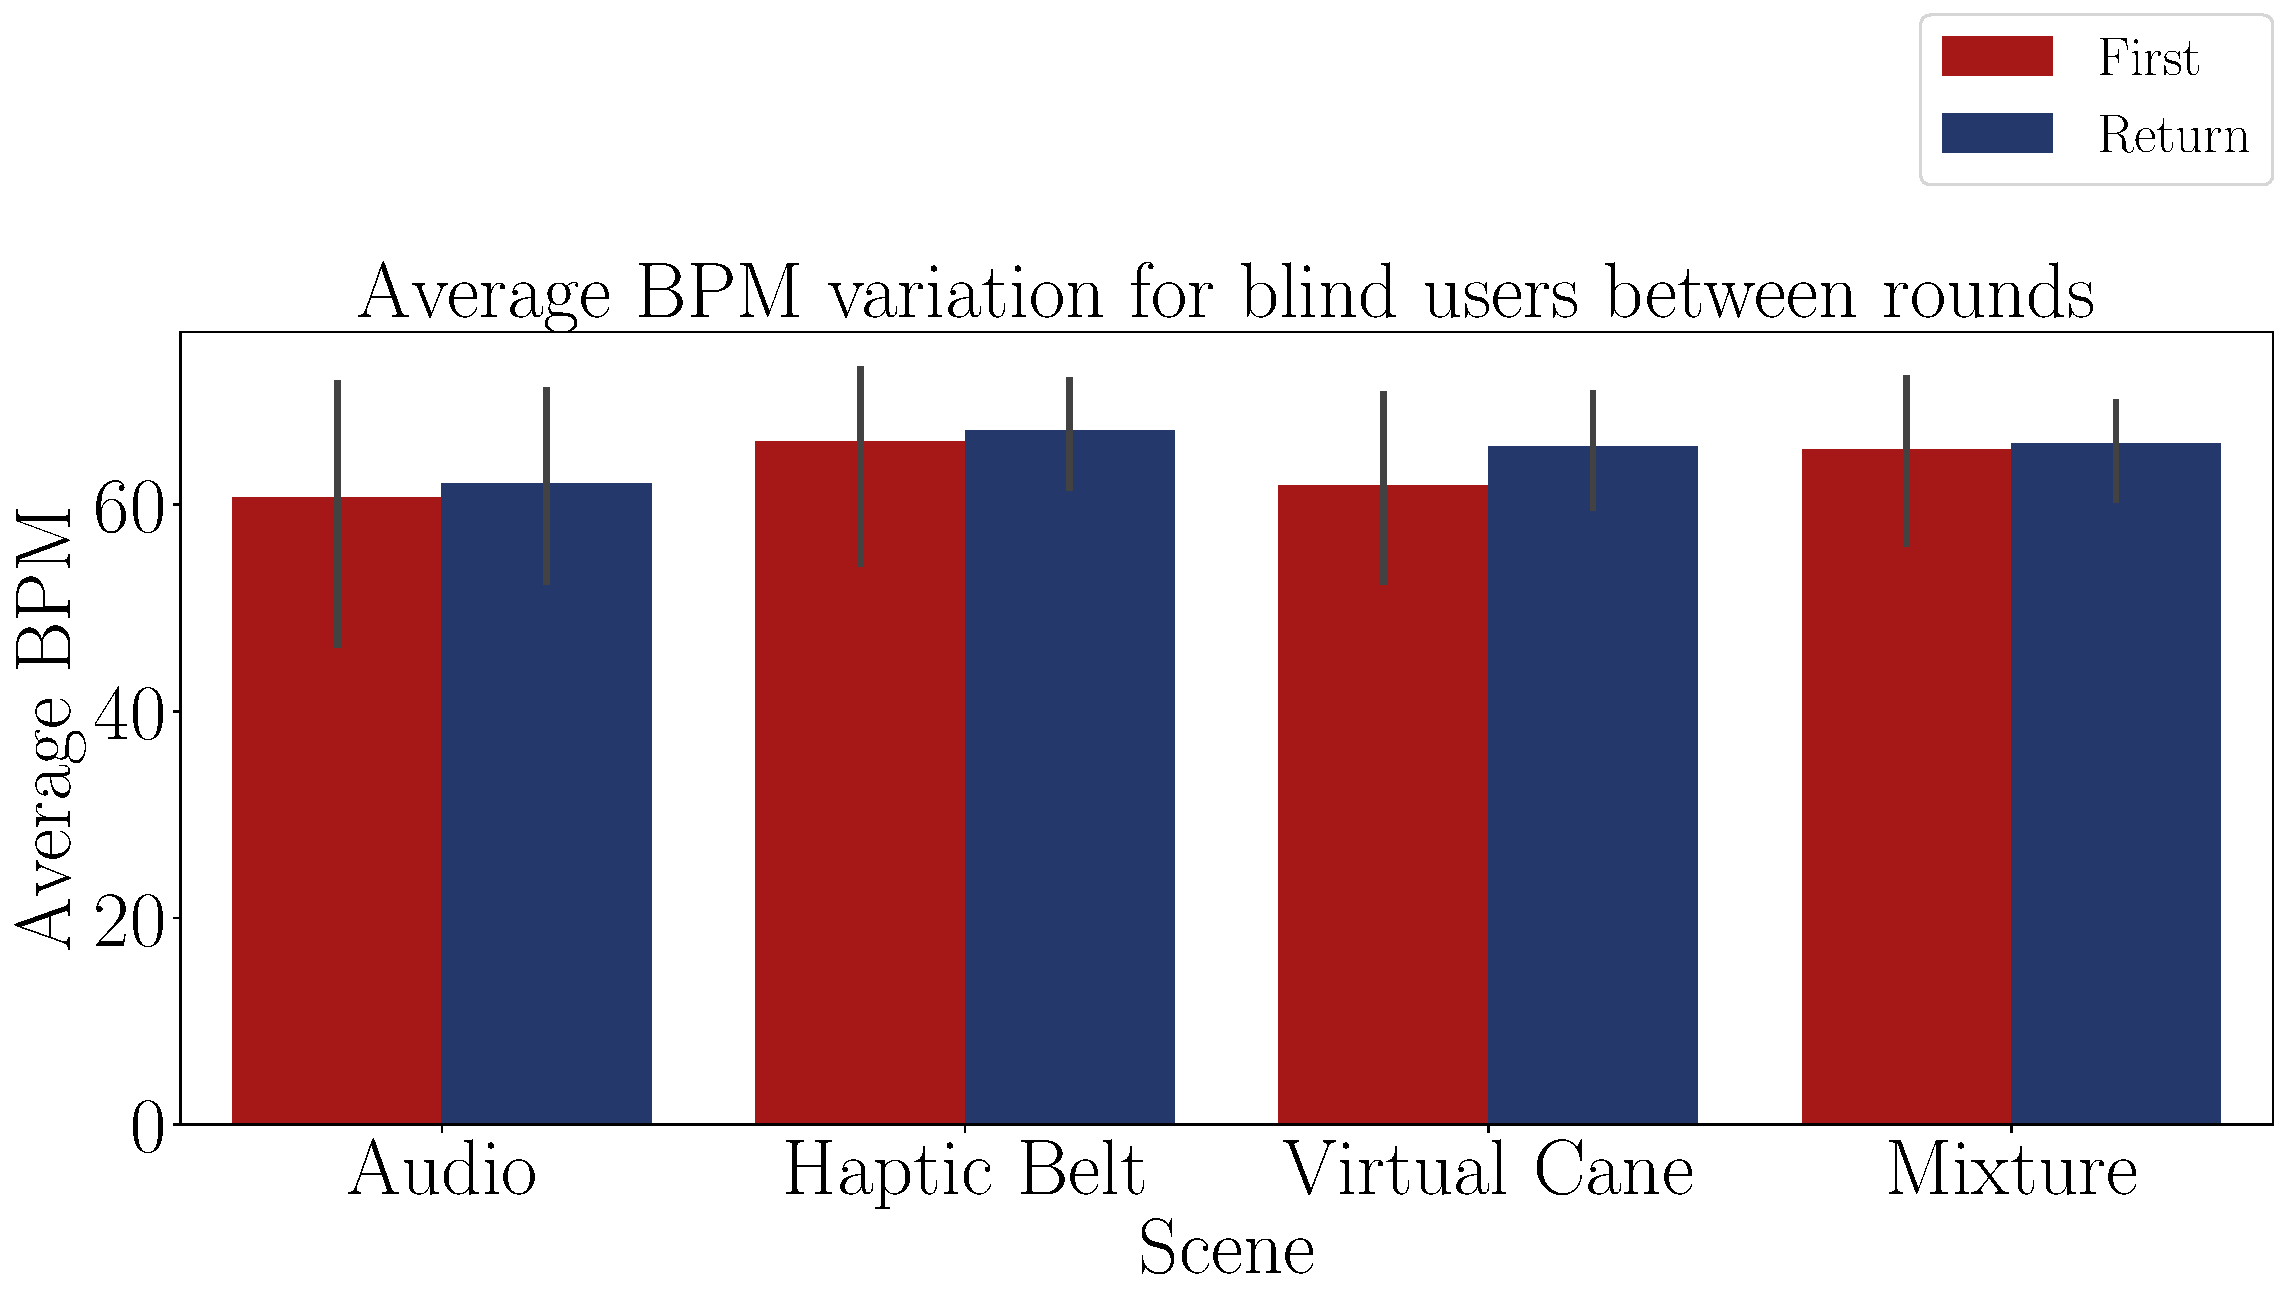
\includegraphics[width = \textwidth]{Resultados/ECG/Figuras/pdf/barplot_ecg_bpm_4_scene_blind.pdf}
        \subcaption{Blind participants.}
        \label{fig:barplot_ecg_bpm_4_scene_blind}
    \end{minipage}
    \begin{minipage}{\textwidth}
        \centering
        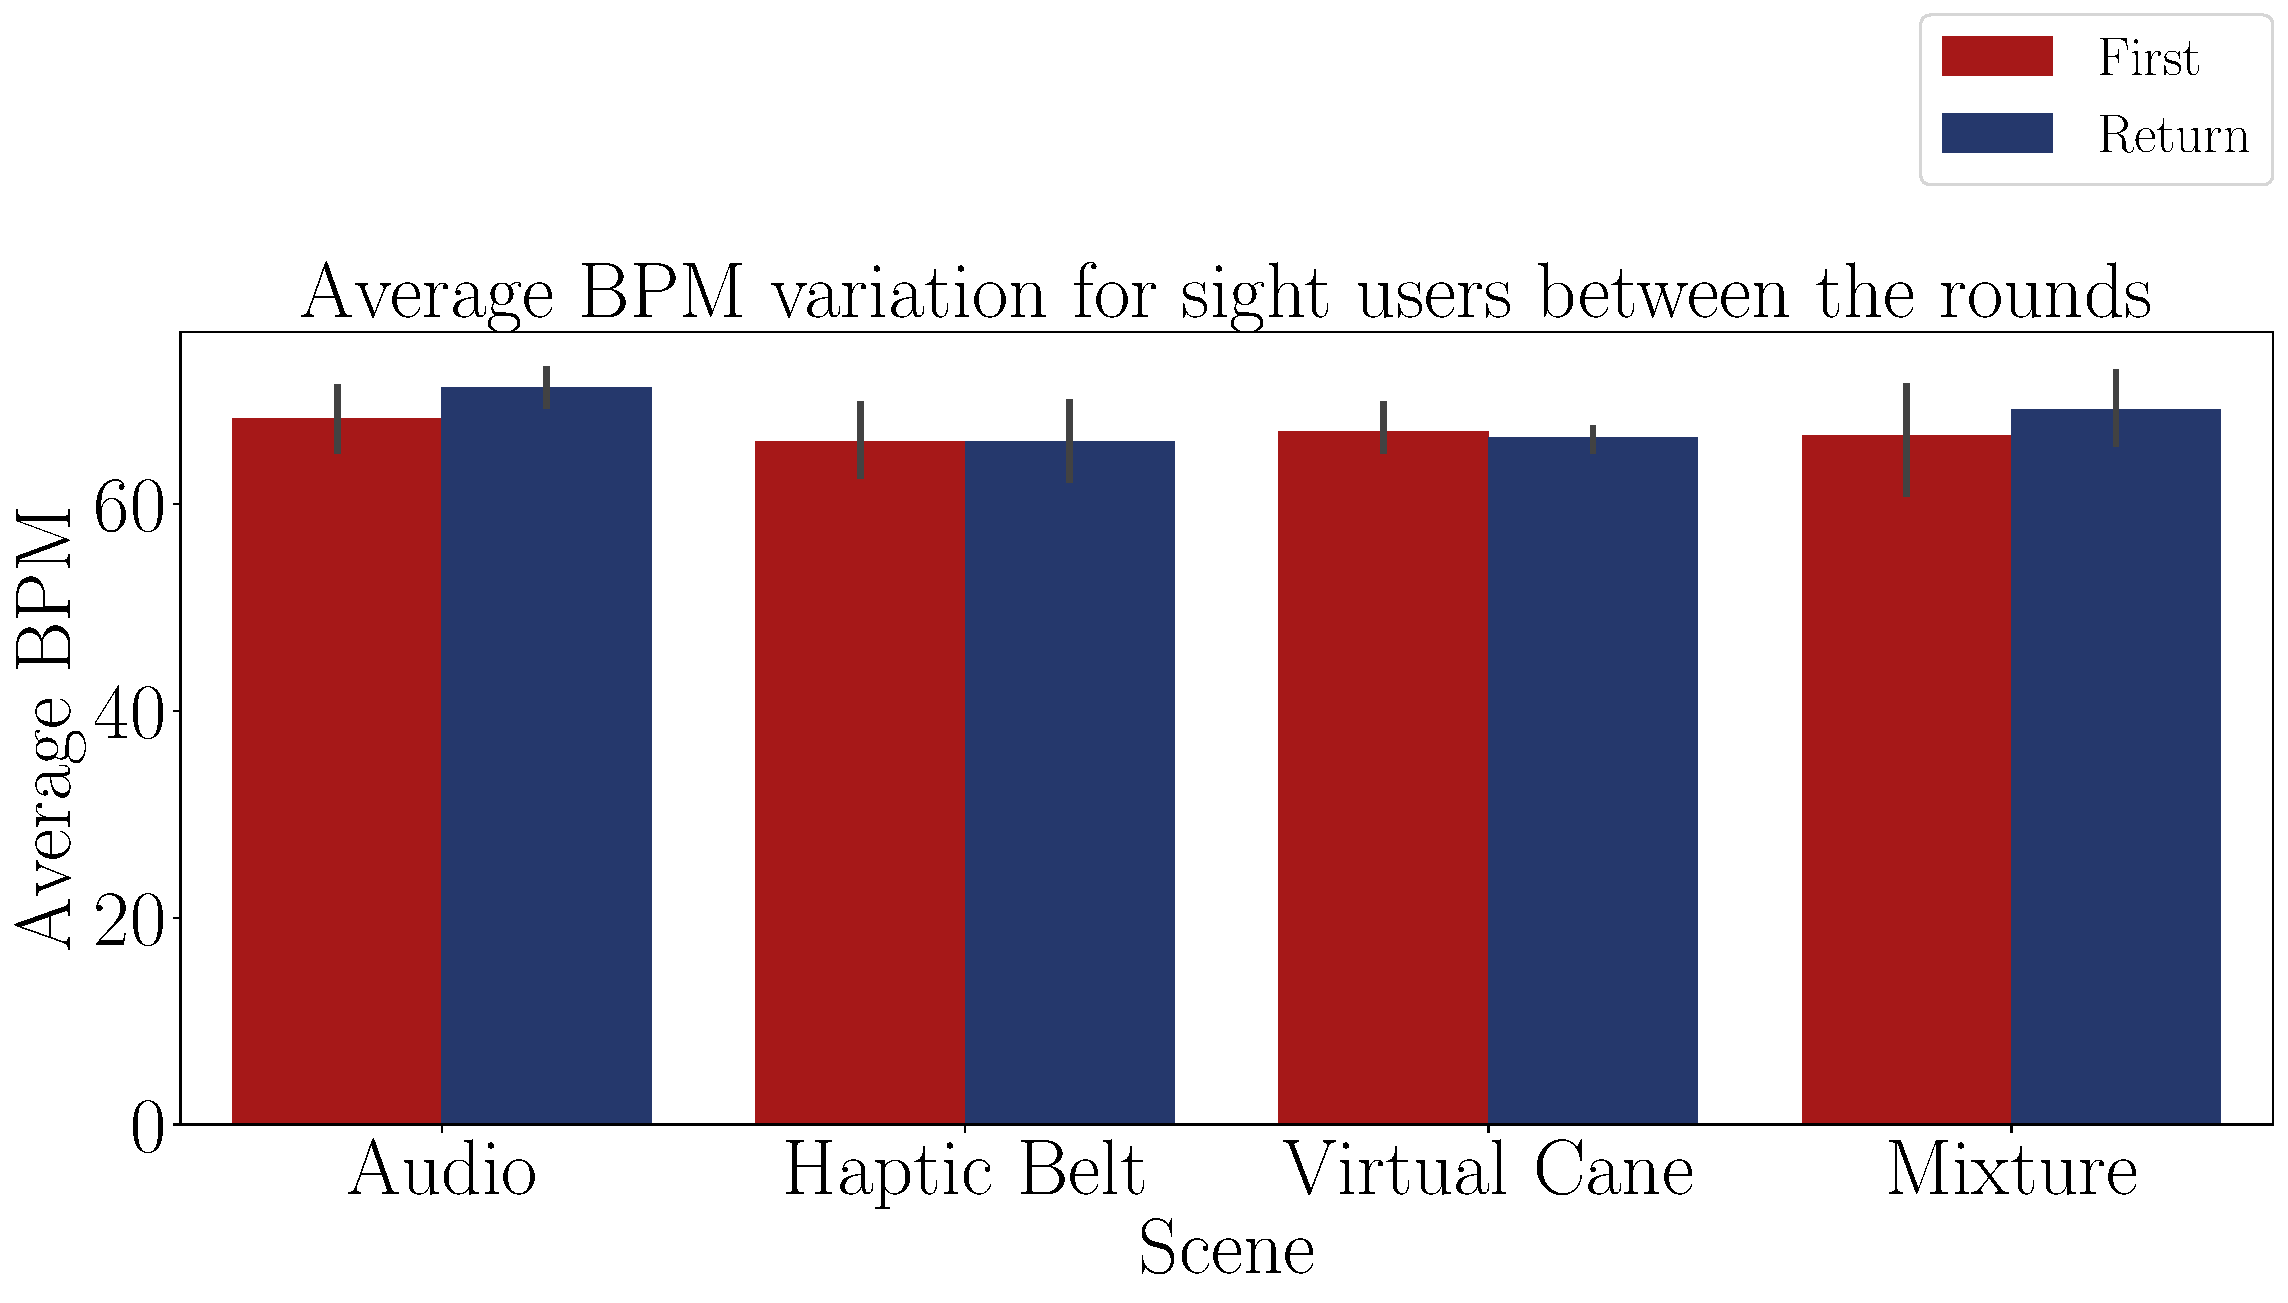
\includegraphics[width = \textwidth]{Resultados/ECG/Figuras/pdf/barplot_ecg_bpm_4_scene_sight.pdf}
        \subcaption{Sight participants.}
        \label{fig:barplot_ecg_bpm_4_scene_sight}
    \end{minipage}
    \caption{Barplot of the average BPM of the on each method and each round.}
    \label{fig:barplot_ecg_bpm_4_scene_blind_sight}
\end{figure}
%\begin{figure}[!htpb]
%    \centering
%    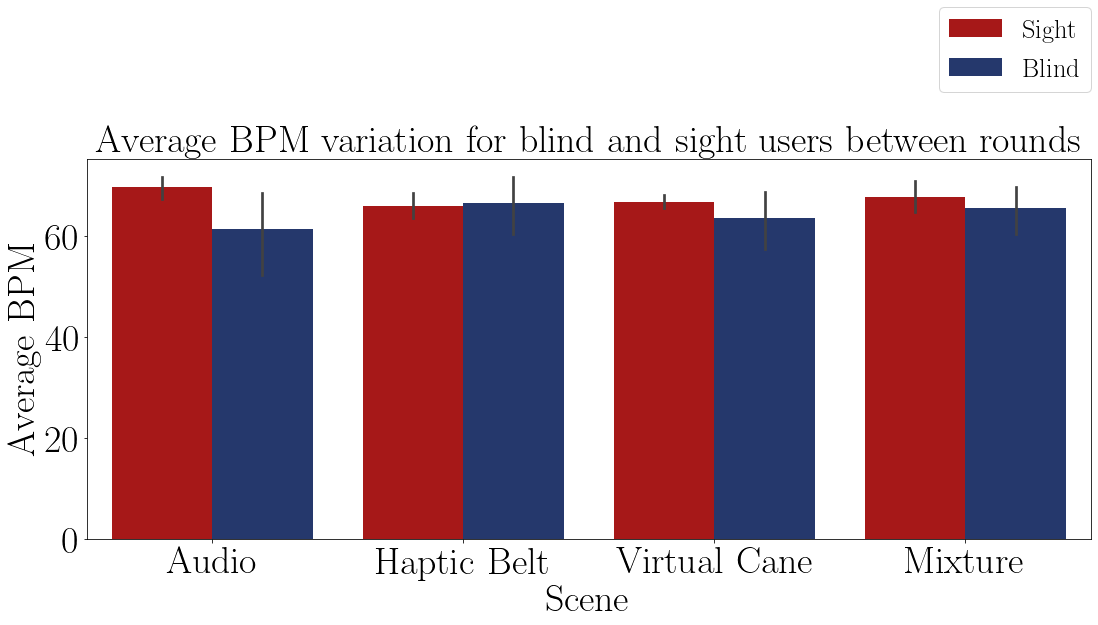
\includegraphics[width = 0.8\linewidth]{Resultados/ECG/Figuras/pdf/barplot_ecg_bpm_4_scene.pdf}
%    \caption{Barplot of the average BPM of both participants on each method.}
%    \label{fig:barplot_ecg_bpm_4_scene}
%\end{figure}

\begin{figure}[!htb]
    \centering
    \begin{minipage}{0.45\textwidth}
        \centering
        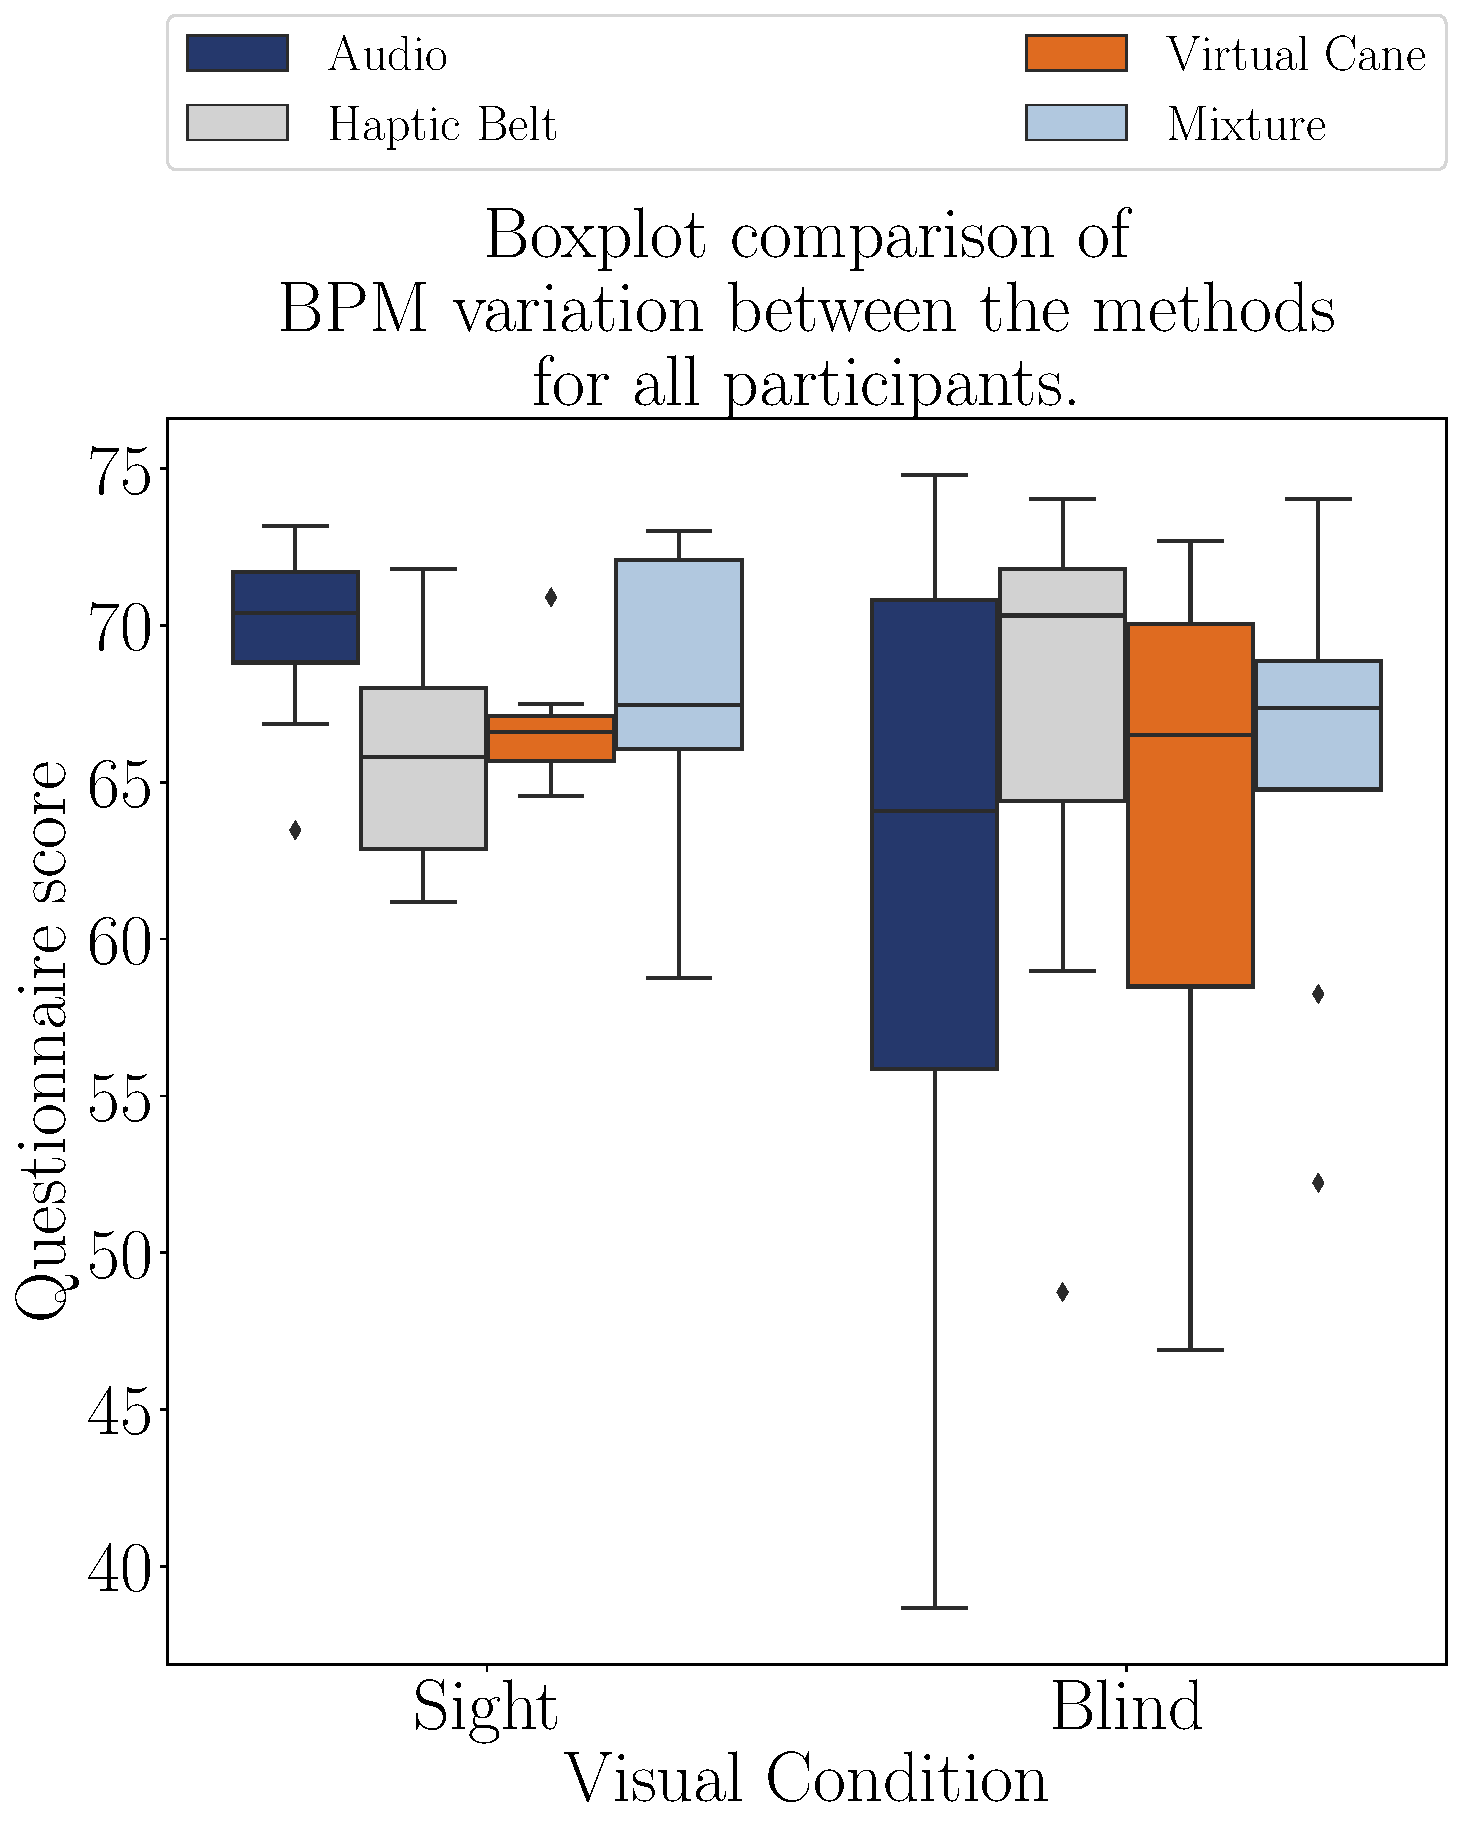
\includegraphics[width = \textwidth]{Resultados/ECG/Figuras/pdf/boxplot_ecg_bpm_4_scene.pdf}
        \caption{Boxplot of the average BPM of the participants grouped by the methods.}
        \label{fig:boxplot_ecg_bpm_4_scene}
    \end{minipage}
    \begin{minipage}{0.075\textwidth}
        \hfill
    \end{minipage}
    \begin{minipage}{0.45\textwidth}
        \centering
        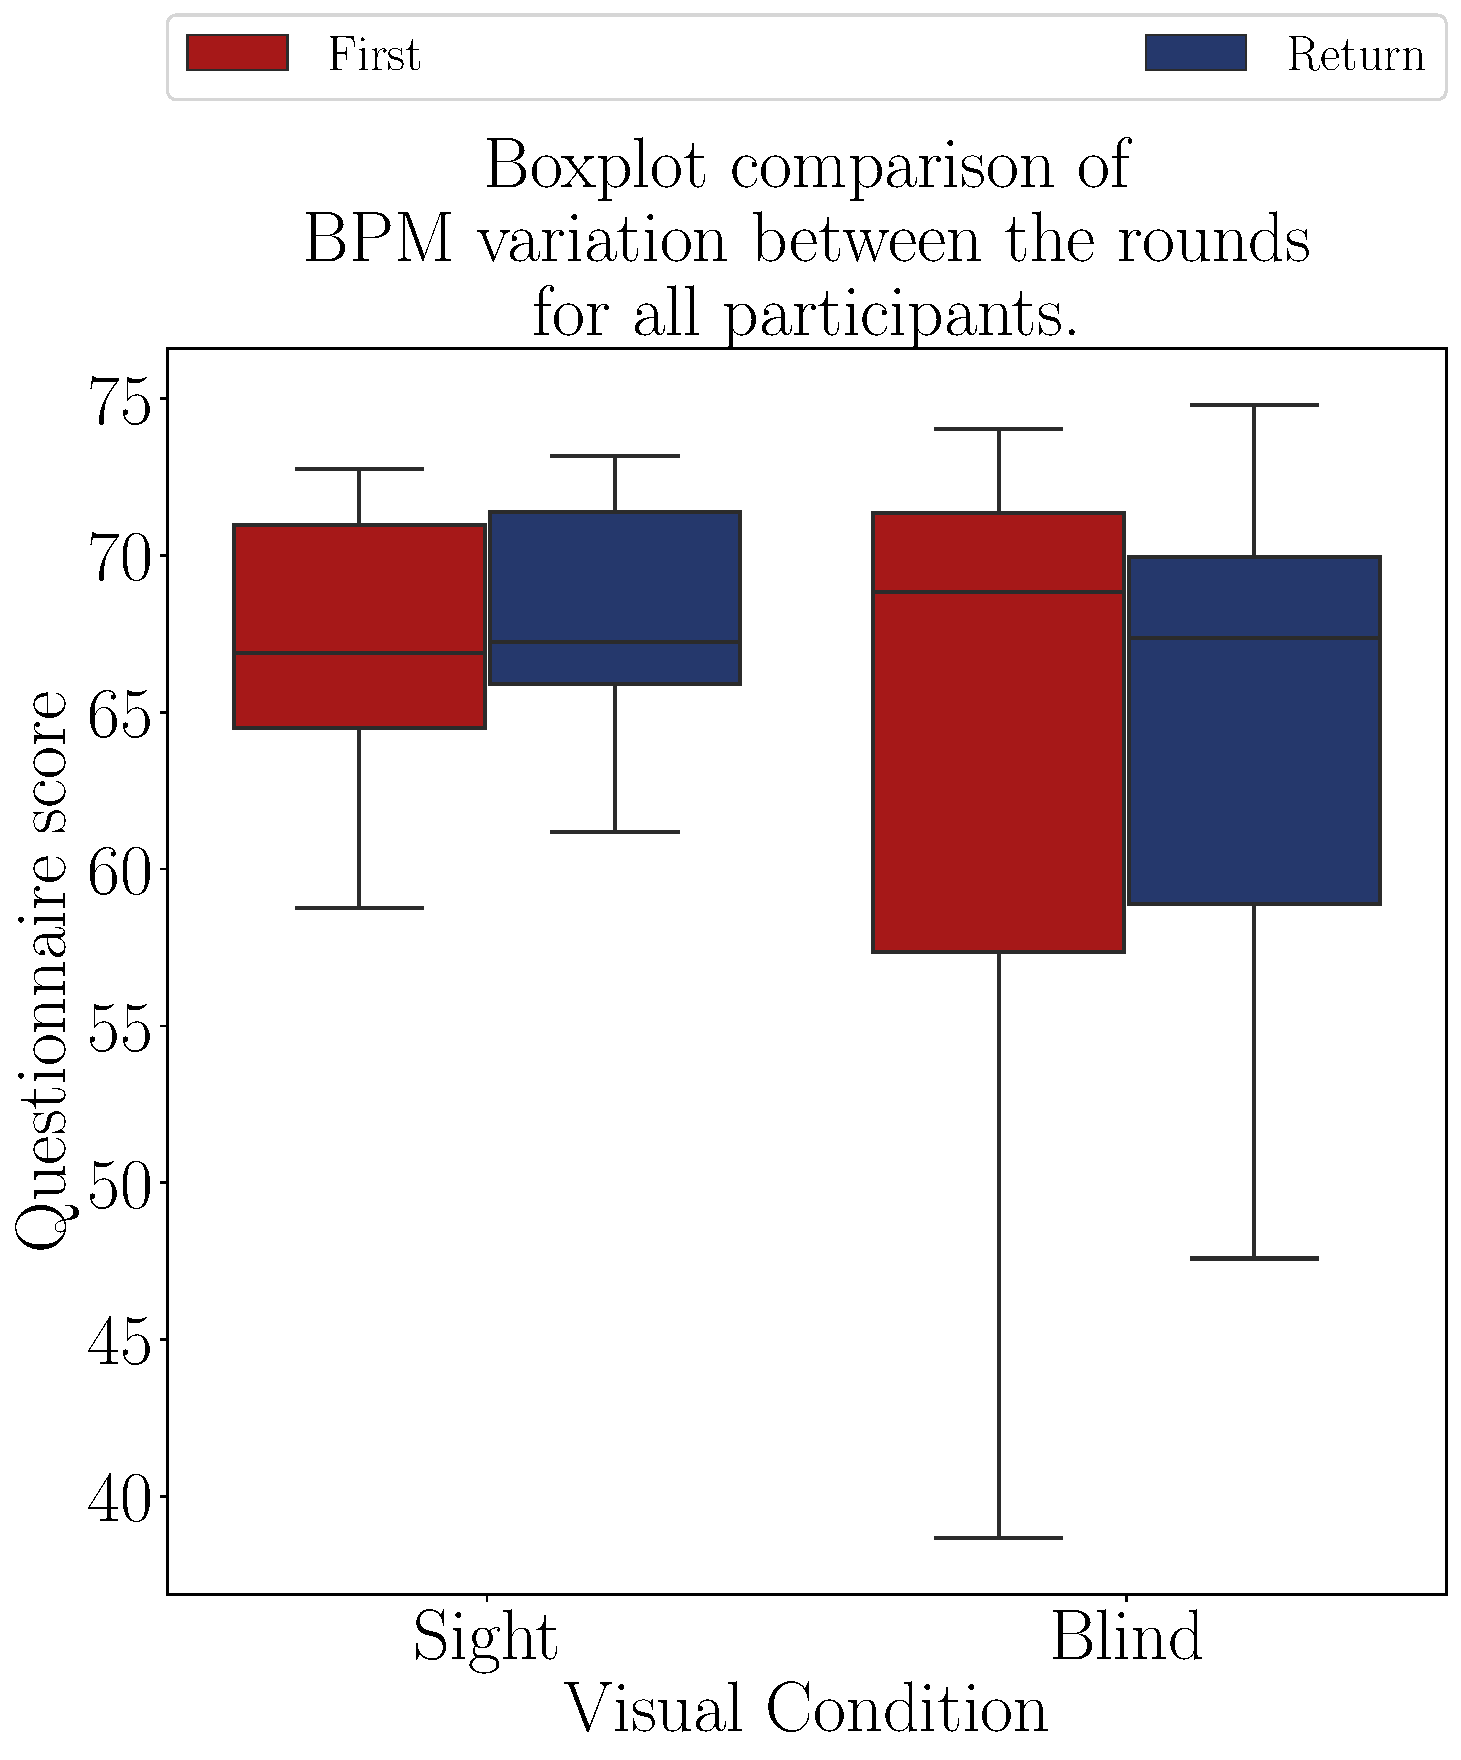
\includegraphics[width = \textwidth]{Resultados/ECG/Figuras/pdf/boxplot_ecg_bpm_4_rounds.pdf}
        \caption{Boxplot of the average BPM of the participants grouped by the rounds.}
        \label{fig:boxplot_ecg_bpm_4_rounds}
    \end{minipage}
\end{figure}
 
%The Table \ref{tab:bpm_average_group_noBase} shows the average heartrate of both samples and is possible to notice how the average score by the blind users was higher in every method, apart of the "Haptic Belt".
%
%
\begin{table}[!htb]
\centering
\caption{ECG average BPM for each method grouped by visual condition.}
\label{tab:bpm_average_group_noBase}
\begin{tabular}{lllrrrr}
\toprule
{} &  Audio & Haptic Belt & Virtual Cane & Mixture \\
Visual Condition &        &             &              &         \\
\midrule
Blind            &  61.40 &       66.68 &        63.72 &   65.65 \\
Sight            &  69.73 &       66.03 &        66.75 &   67.88 \\
\bottomrule
\end{tabular}
\end{table}



Figures \ref{fig:qqplot_bpm_two_way_sight} and \ref{fig:residplot_bpm_two_way_sight} show the QQ plot and residual distributions for the sighted participants of Table \ref{tab:bpm_table_noBase}. These figures show that the data are normally distributed and that the methods have a similar variance. Table \ref{tab:blocanova_bpm_two_way_blind_sight} brings the results from ANOVA, which are similar for both sighted and blind participants.


\begin{table}[!htb]
    \caption{Anova p-value for the BPM on each method.}
    \label{tab:blocanova_bpm_two_way_blind_sight}
\begin{minipage}{0.45\textwidth}
    \subcaption{Blind participants}
    \input{Resultados/ECG/Tabelas/blocanova_bpm_two_way_blindsemBegin.tex}
\end{minipage}
\begin{minipage}{0.45\textwidth}
    \subcaption{Sight participants}
    \input{Resultados/ECG/Tabelas/blocanova_bpm_two_way_sightsemBegin.tex}
\end{minipage}
\end{table}

\begin{figure}[!htb]
    \centering
    %\vspace{-15.0cm}
    \begin{minipage}{0.45\textwidth}
        \centering
        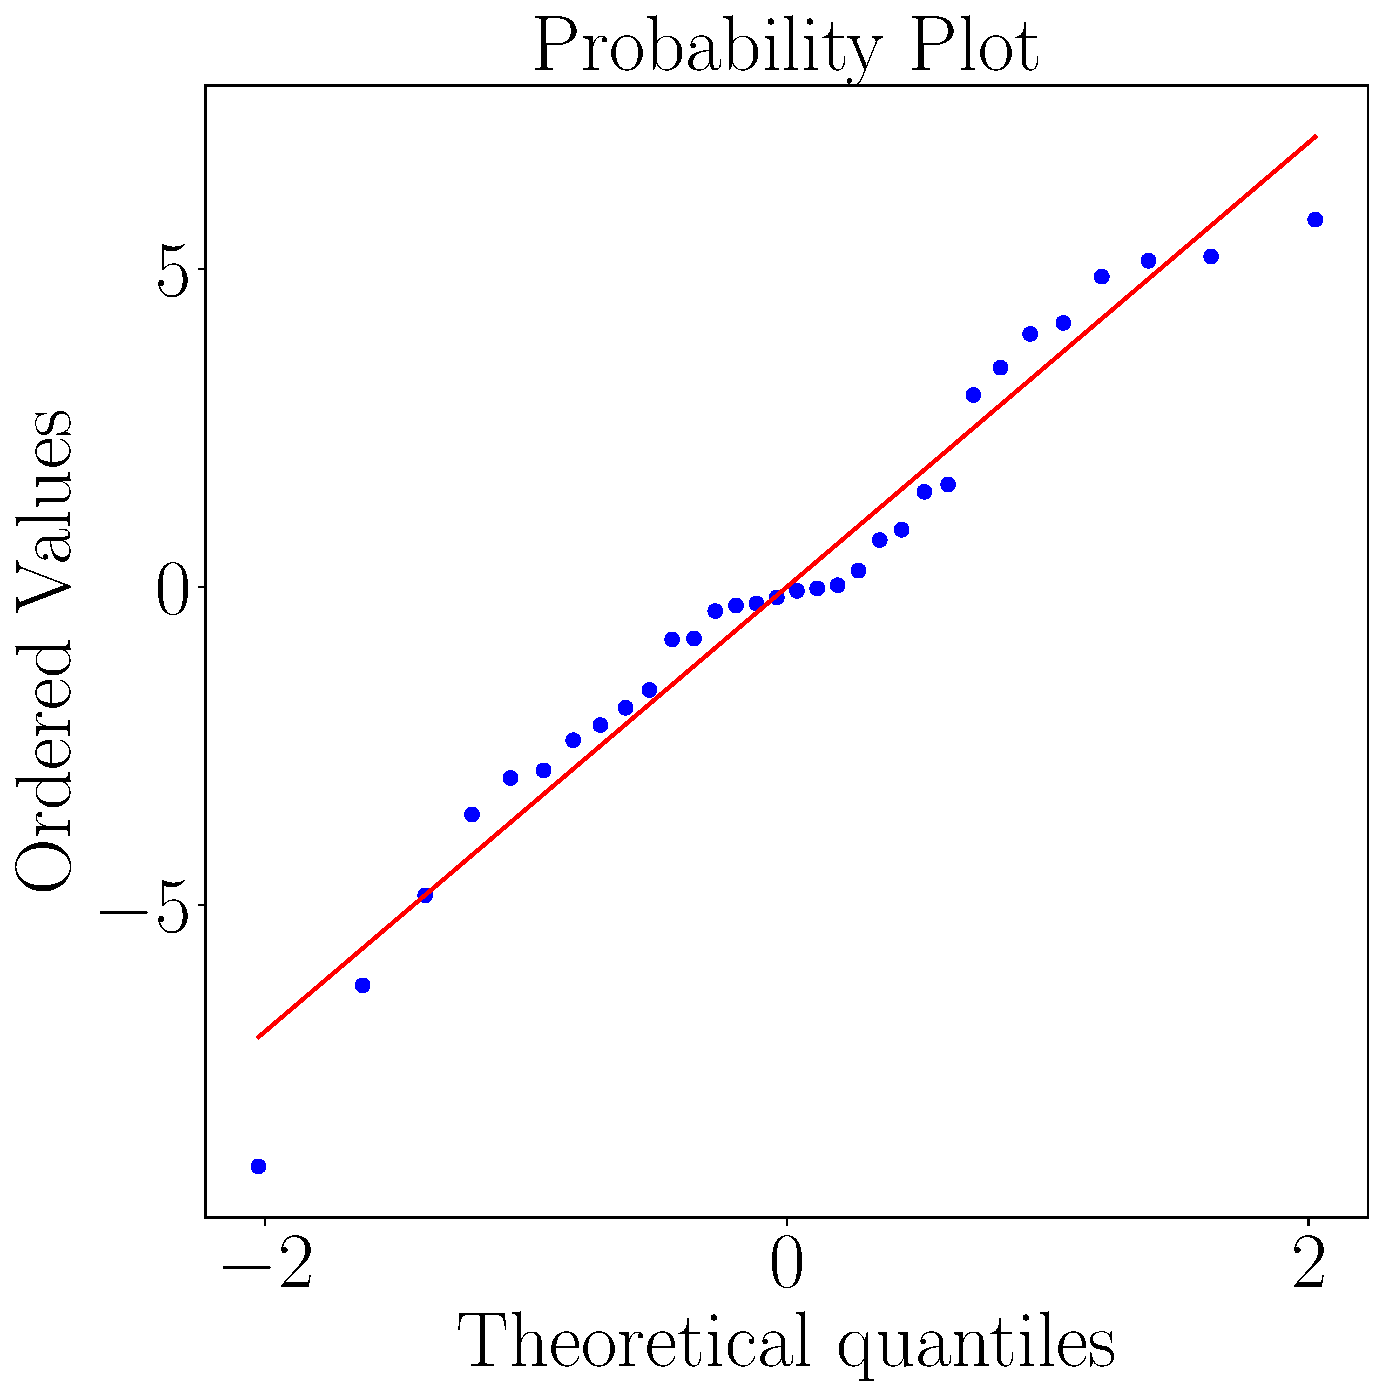
\includegraphics[width = \textwidth]{Resultados/ECG/Figuras/pdf/qqplot_bpm_two_way_sight.pdf}
        \caption{QQ plot of the BPM of the sight participants on each method.}
        \label{fig:qqplot_bpm_two_way_sight}
    \end{minipage}
    \begin{minipage}{0.075\textwidth}
        \hfill
    \end{minipage}
    \begin{minipage}{0.45\textwidth}
        \centering
        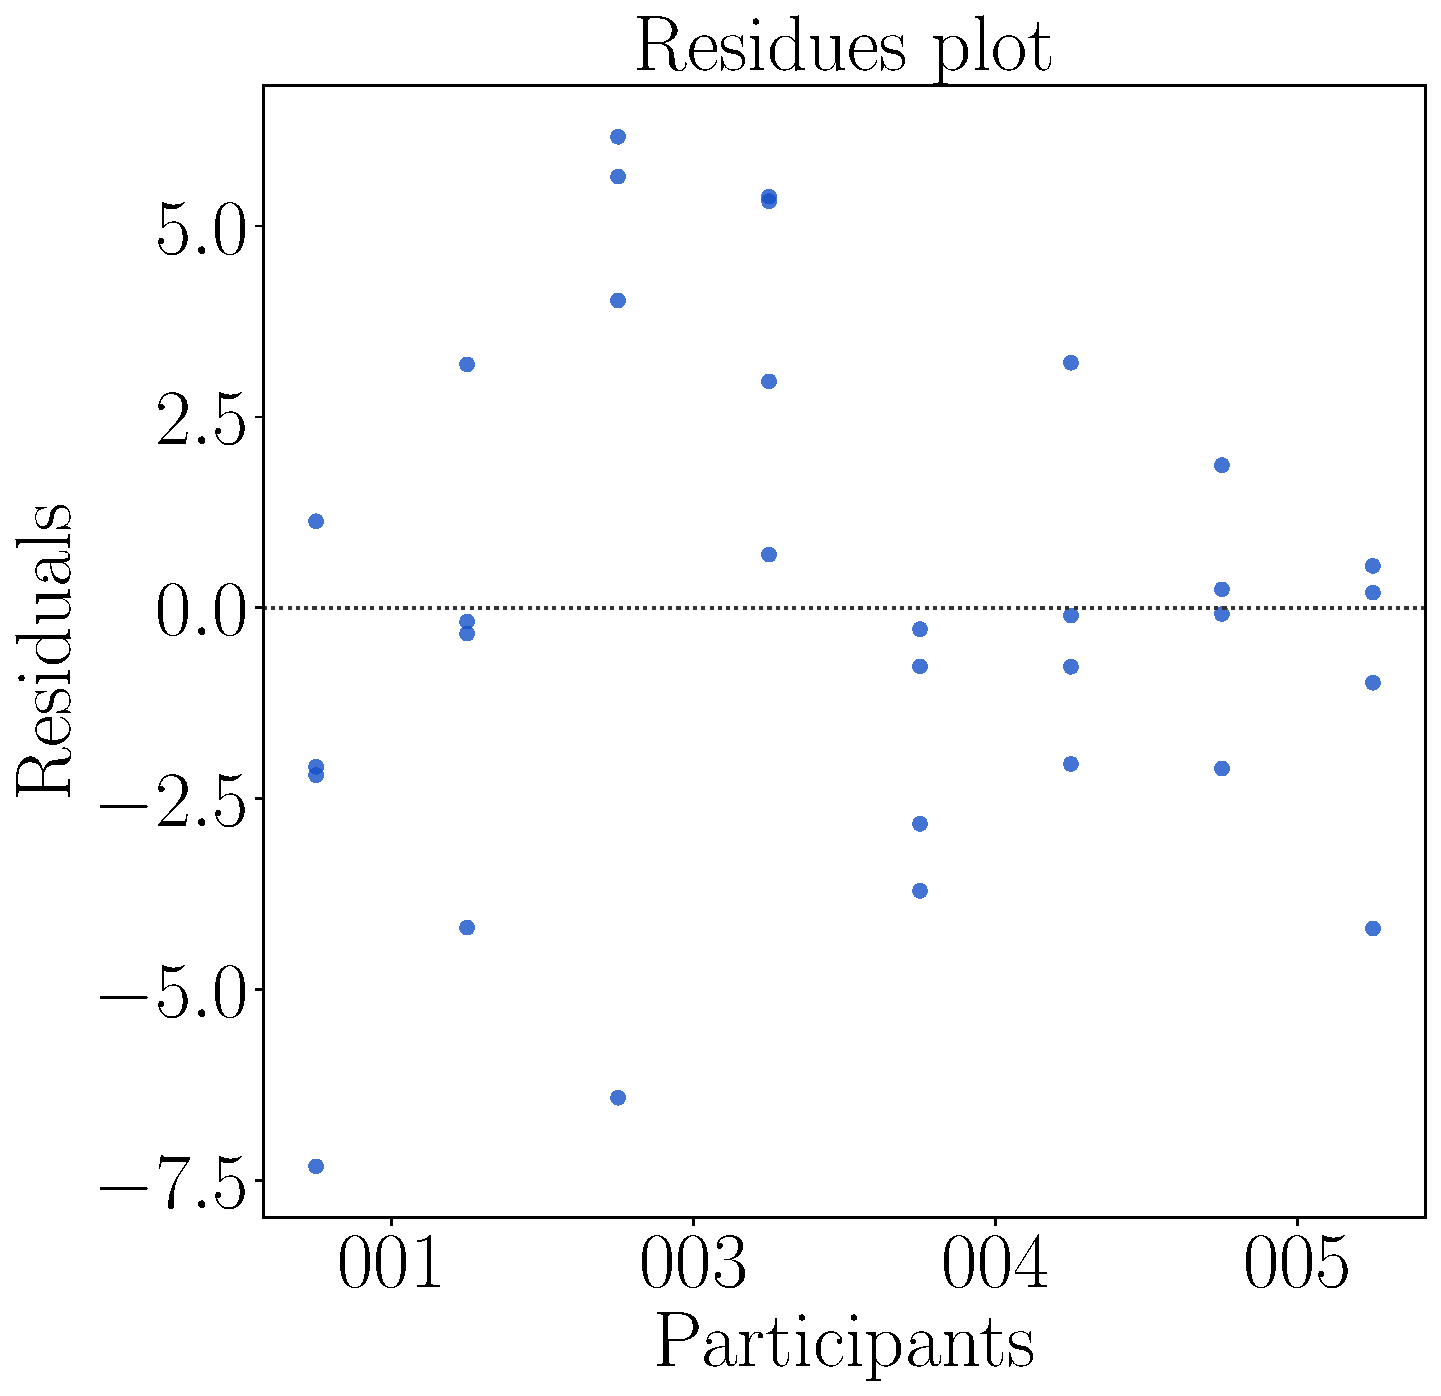
\includegraphics[width = \textwidth]{Resultados/ECG/Figuras/pdf/residplot_bpm_two_way_sight.pdf}
        \caption{Residual plot of the BPM score the sight participants on each method.}
        \label{fig:residplot_bpm_two_way_sight}
    \end{minipage}
\end{figure}

%
\begin{table}[!htb]
\centering
\caption{Cross validation p-value for the average BPM on each method for blinded users.}
\label{tab:lsd_bpm_two_way_sight}
\begin{tabular}{rclr}
\toprule
      \multicolumn{3}{c}{Method} &                          \multicolumn{2}{c}{Analysis} \\
\midrule
       Audio & $X$ & Haptic Belt &        $H_1 : \mu_{Audio} \ne \mu_{Haptic Belt}$ & ** \\
      Audio & $X$ & Virtual Cane &       $H_1 : \mu_{Audio} \ne \mu_{Virtual Cane}$ & ** \\
           Audio & $X$ & Mixture &            $H_1 : \mu_{Audio} \ne \mu_{Mixture}$ & ** \\
Haptic Belt & $X$ & Virtual Cane & $H_1 : \mu_{Haptic Belt} \ne \mu_{Virtual Cane}$ & ** \\
     Haptic Belt & $X$ & Mixture &      $H_1 : \mu_{Haptic Belt} \ne \mu_{Mixture}$ & ** \\
    Virtual Cane & $X$ & Mixture &     $H_1 : \mu_{Virtual Cane} \ne \mu_{Mixture}$ & ** \\
\bottomrule
\end{tabular}
\end{table}



%The Table \ref{tab:lsd_bpm_two_way_sight} presents the conclusion of a pairwise Fisher LSD test of the blind heart rate frequency variation between all the guidance methods and it shows that all methods had different effect on the heartrate.

%According to the ANOVA test at Table \ref{tab:blocanova_bpm_two_way_sight} there was no effect of the methods neither the rounds or their interaction, despite the fact that the Figure \ref{fig:boxplot_ecg_bpm_4_scene} showed a big difference between the methods. So the methods did not influence the sighted user mental workload. The same conclusion was driven in the section \ref{subsubsec:results_ecg_1} in the BPM part.

\FloatBarrier

%%%%%%%%%%%%%%%%%%%%%%%%%%%%%%%%%%%%%%%%%%%%%%%%%%%%%%%%%%%%%%%%%%%%%%%%%%%%
%%%%%%%%%%%%%%%%%%%%%%%%%%%%%%%%%%%%%%%%%%%%%%%%%%%%%%%%%%%%%%%%%%%%%%%%%%%%
%%%%%%%%%%%%%%%%%%%%%%%%%%%%%%%%%%%%%%%%%%%%%%%%%%%%%%%%%%%%%%%%%%%%%%%%%%%%
%%%%%%%%%%%%%%%%%%%%%%%%%%%%%%%%%%%%%%%%%%%%%%%%%%%%%%%%%%%%%%%%%%%%%%%%%%%%
%
%
\paragraph{Analysis of the heartbeat variance (SDNN)}\mbox{}\\
%

Table \ref{tab:sdnn_table_noBase} presents the SDNN for both sighted and blind participants. Different to the heartrate frequency, if the variation between the First and the Return round is negative, it means that the user had an increase on his/her mental workload and vice-versa. The mean values are presented in the barplots of Figure \ref{fig:barplot_ecg_sdnn_4_scene_blind_sight}.


\begin{table}[!htb]
\centering
\caption{Average SDNN by the participants during the each round and method [ms].}
\label{tab:sdnn_table_noBase}
\begin{tabular}{lllrrrrr}
\toprule
    &       &        &   Audio &  \begin{tabular}[c]{@{}l@{}}Haptic\\ Belt\end{tabular} &  \begin{tabular}[c]{@{}l@{}}Virtual\\ Cane\end{tabular} &  Mixture \\
Part. & \begin{tabular}[c]{@{}l@{}}Visual\\ Condition\end{tabular} & Round &         &                                                        &                                                         &          \\
\midrule
001C & Blind & First & 107.061 &                                                124.737 &                                                 163.968 &  129.054 \\
    &       & Return & 130.885 &                                                131.590 &                                                 157.589 &  124.786 \\
002C & Blind & First &  98.863 &                                                 81.140 &                                                  33.977 &   79.289 \\
    &       & Return &  49.627 &                                                 42.815 &                                                 114.057 &  107.545 \\
003C & Blind & First &  38.325 &                                                 35.101 &                                                  42.392 &   43.692 \\
    &       & Return &  41.196 &                                                 44.256 &                                                  42.602 &   46.145 \\
004C & Blind & First &  86.827 &                                                 62.560 &                                                  85.900 &   70.472 \\
    &       & Return &  74.895 &                                                 70.017 &                                                  66.089 &  104.040 \\
001 & Sight & First &  82.185 &                                                134.530 &                                                 134.773 &  225.408 \\
    &       & Return &  69.479 &                                                318.747 &                                                 116.003 &  136.507 \\
003 & Sight & First &  79.600 &                                                 51.782 &                                                  68.676 &   60.842 \\
    &       & Return &  45.709 &                                                 40.927 &                                                  66.323 &   47.823 \\
004 & Sight & First & 121.130 &                                                154.718 &                                                 128.477 &  125.947 \\
    &       & Return & 100.366 &                                                122.563 &                                                 140.115 &  119.260 \\
005 & Sight & First &  87.686 &                                                120.522 &                                                  88.591 &  102.796 \\
    &       & Return &  93.207 &                                                122.839 &                                                 141.305 &   96.035 \\
\bottomrule
\end{tabular}
\end{table}



\begin{figure}[!htpb]
    \centering
    \begin{minipage}{\textwidth}
        \centering
        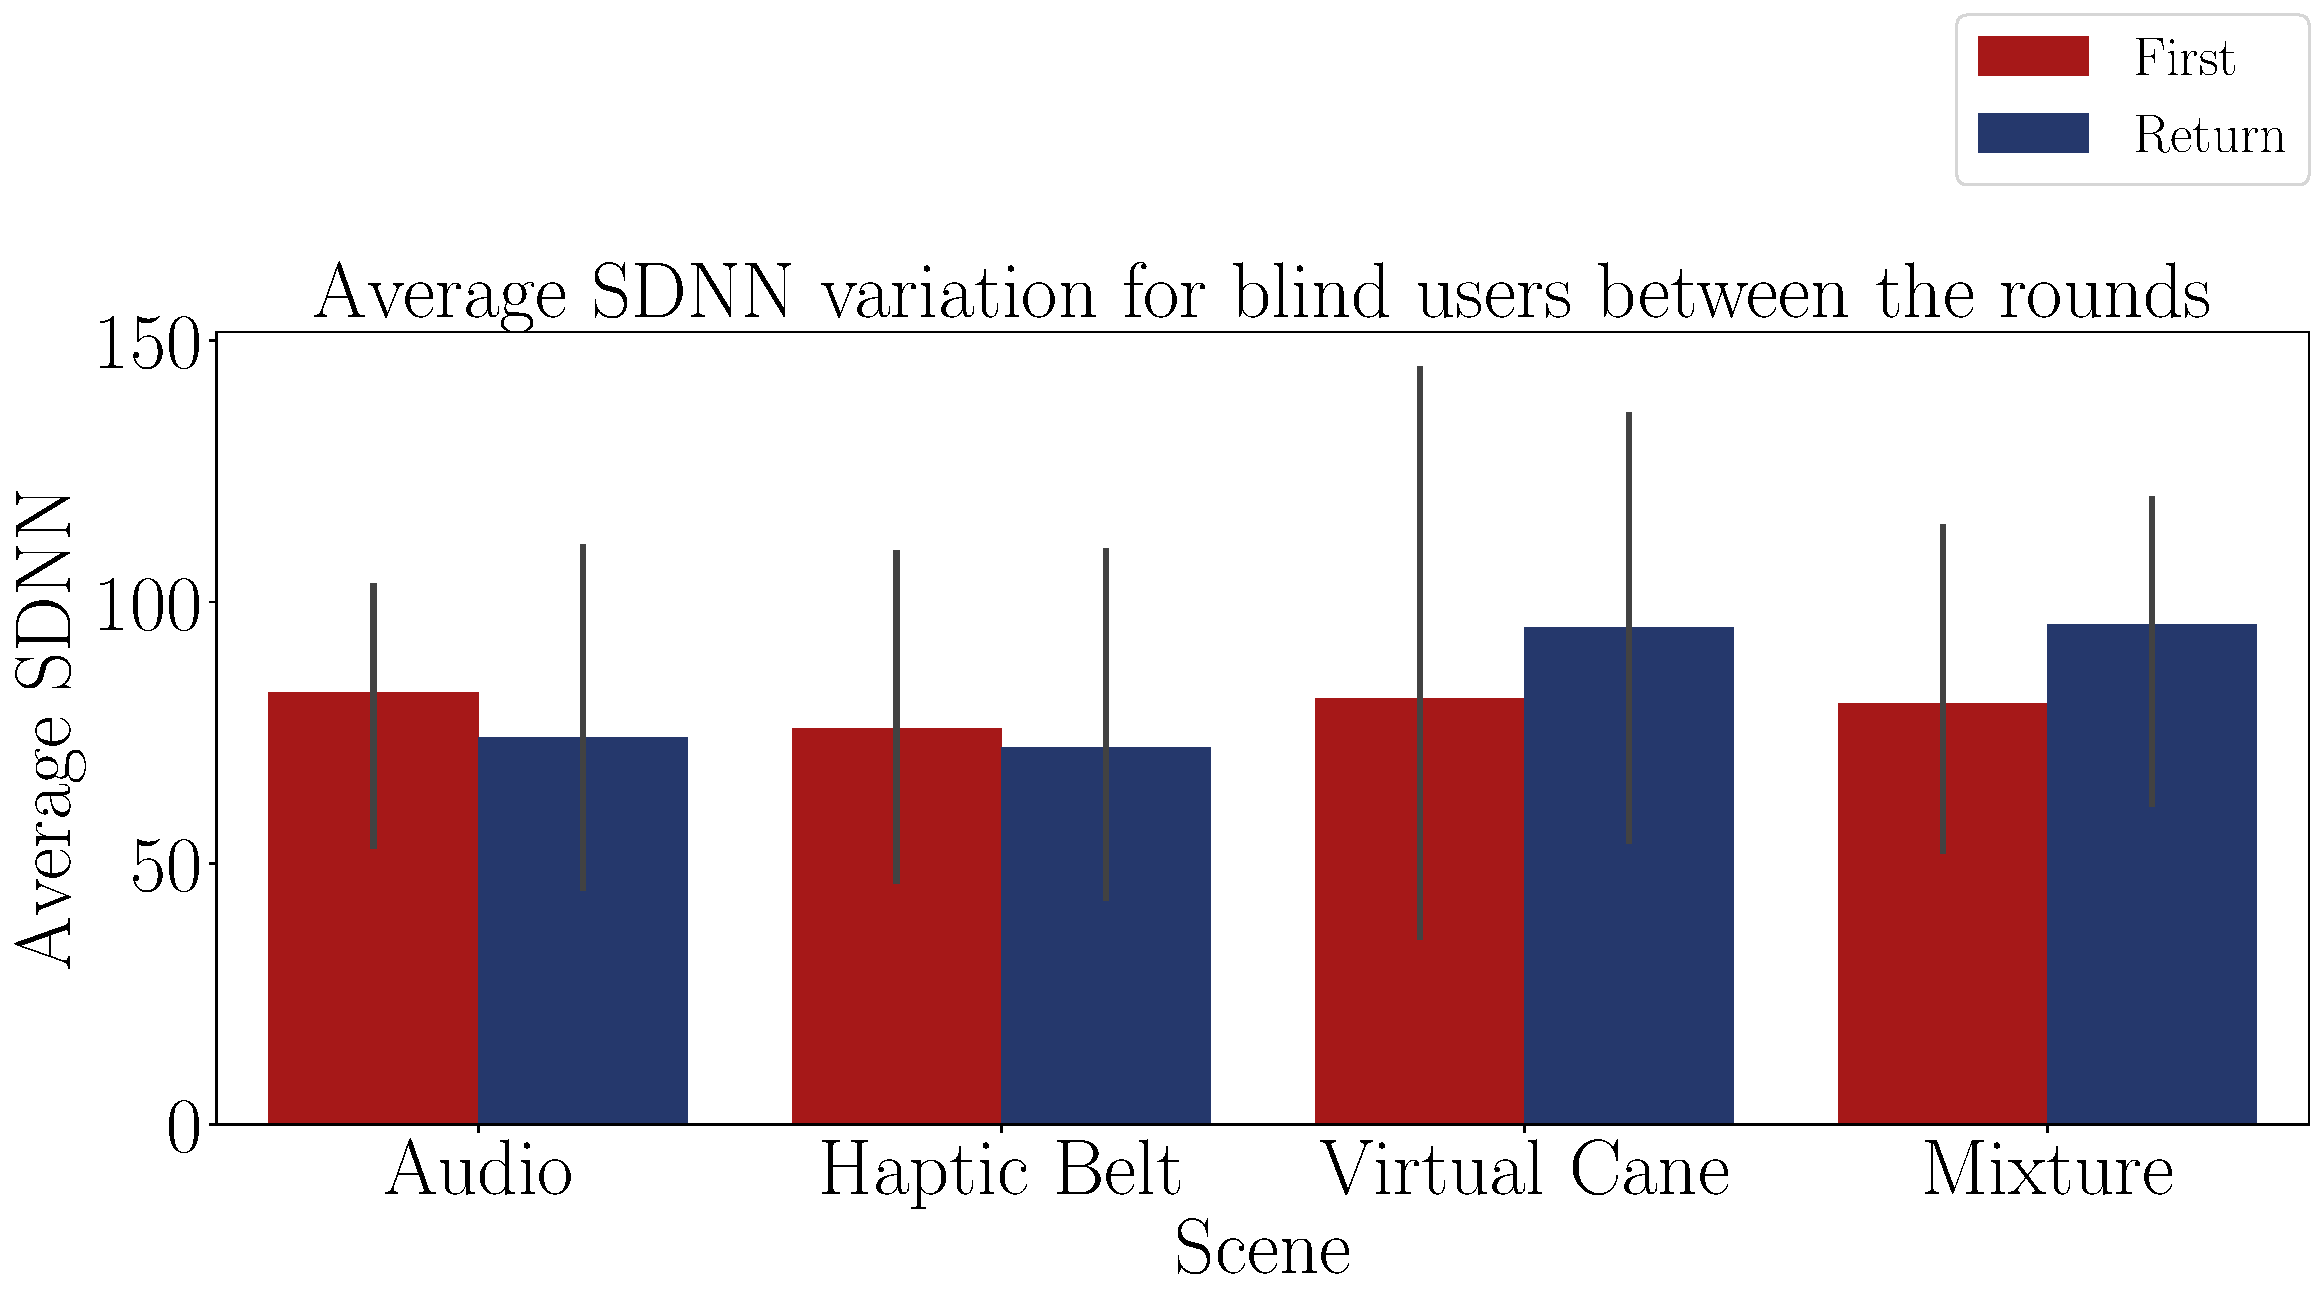
\includegraphics[width = \textwidth]{Resultados/ECG/Figuras/pdf/barplot_ecg_sdnn_4_scene_blind.pdf}
        \subcaption{Blind participants.}
        \label{fig:barplot_ecg_sdnn_4_scene_blind}
    \end{minipage}
    \begin{minipage}{\textwidth}
        \centering
        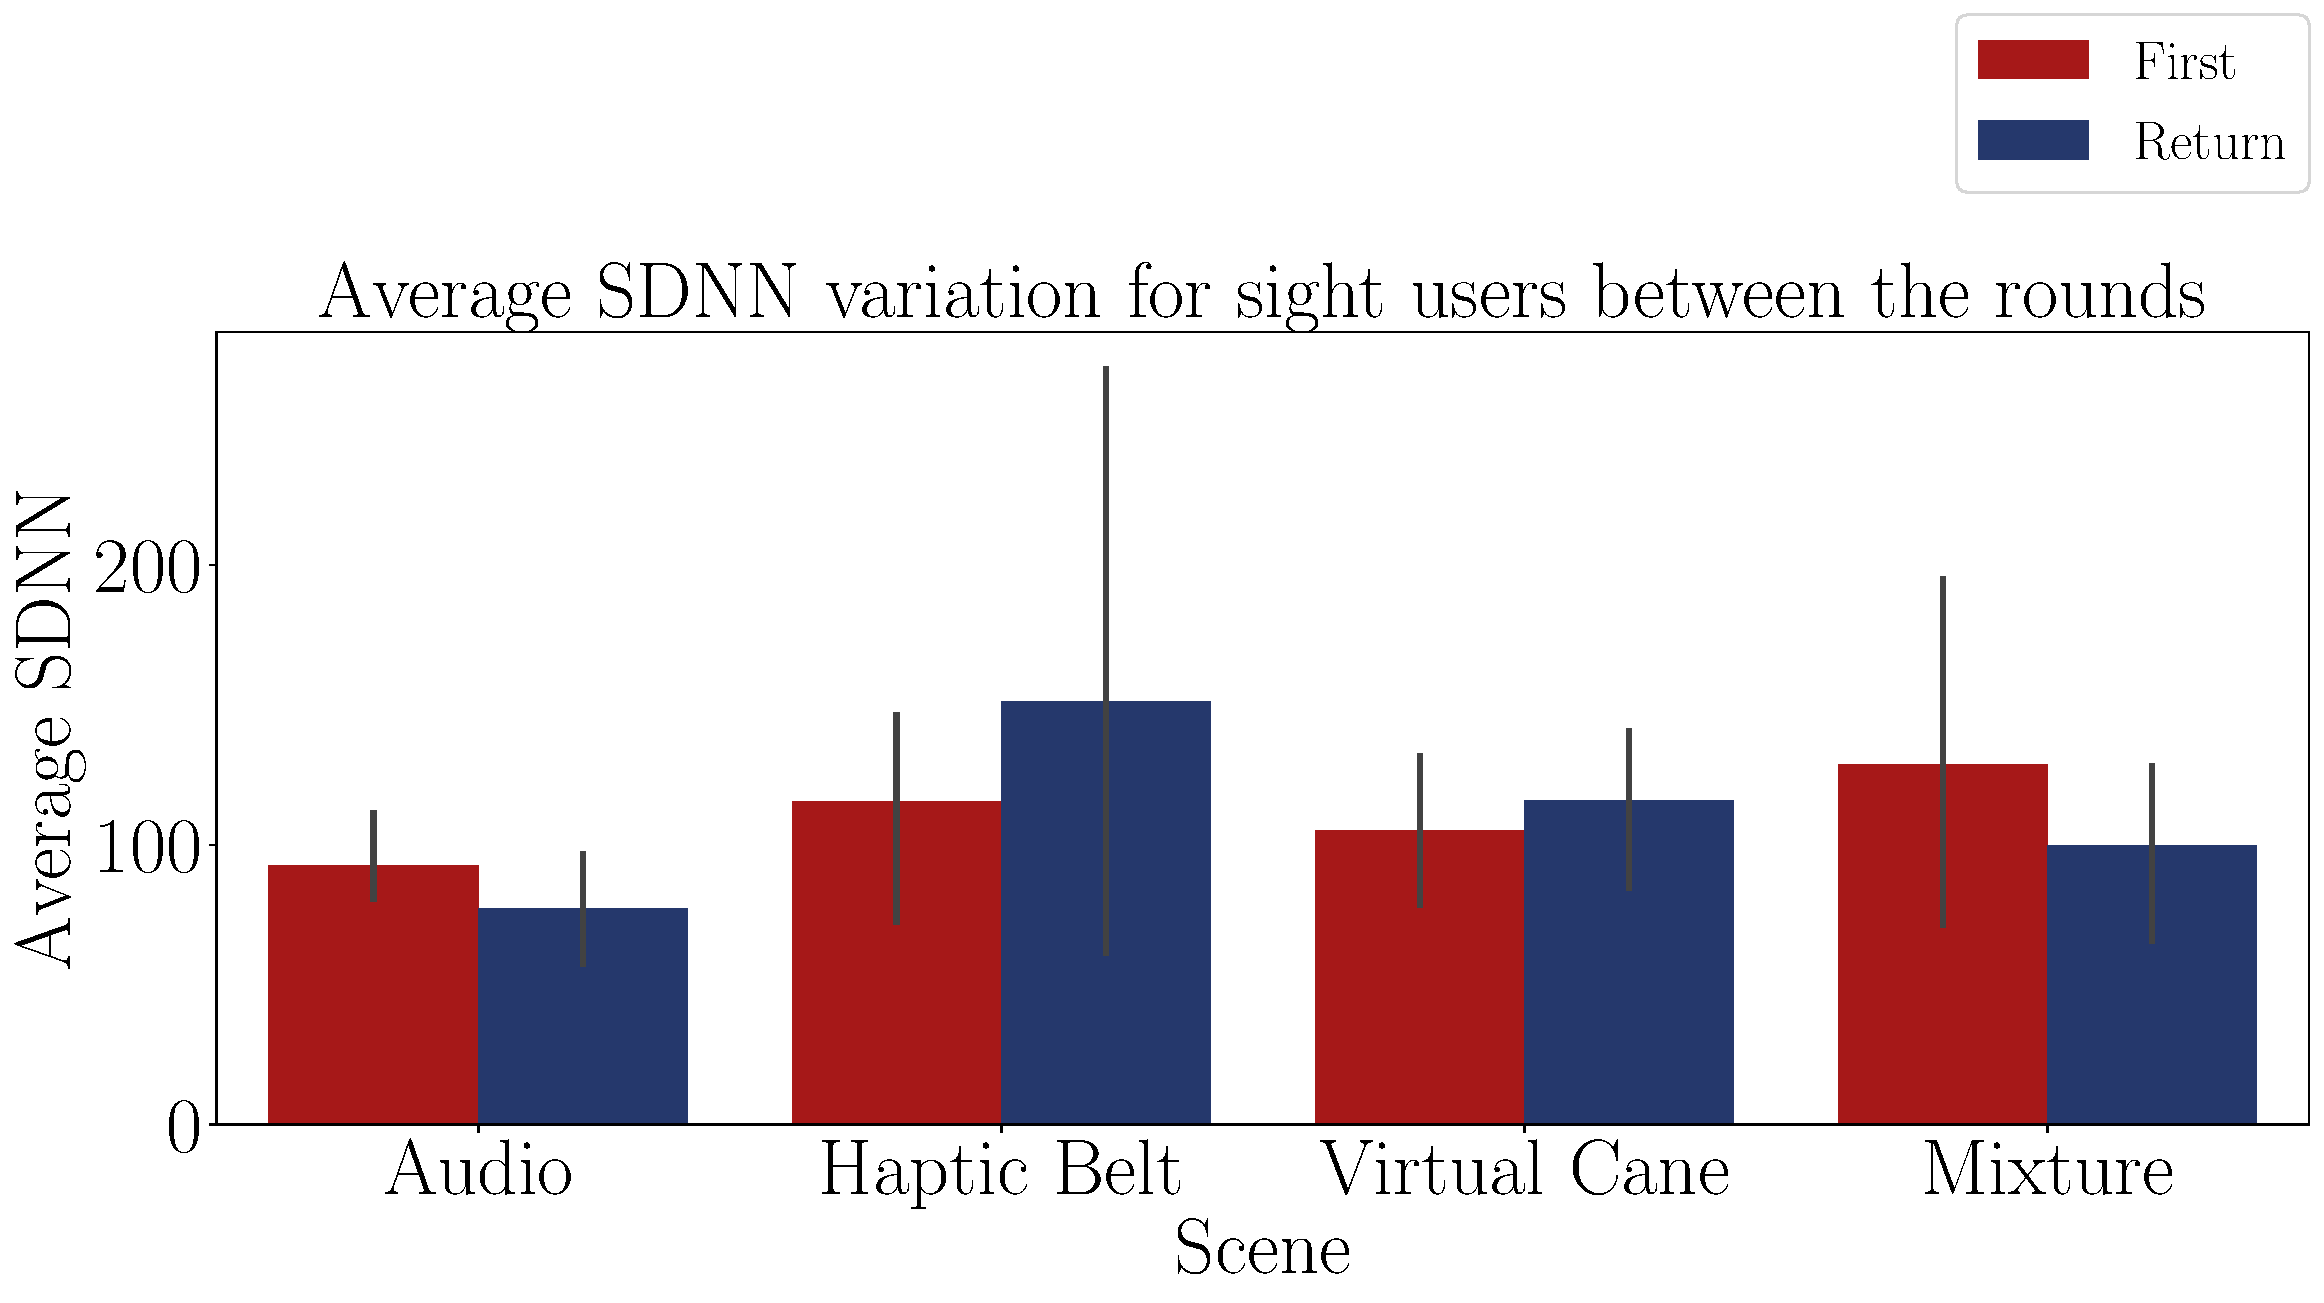
\includegraphics[width = \textwidth]{Resultados/ECG/Figuras/pdf/barplot_ecg_sdnn_4_scene_sight.pdf}
        \subcaption{Sight participants.}
        \label{fig:barplot_ecg_sdnn_4_scene_sight}
    \end{minipage}
    \caption{Barplot of the average SDNN of the on each method and round.}
    \label{fig:barplot_ecg_sdnn_4_scene_blind_sight}
\end{figure}
%\begin{figure}[!htpb]
%    \centering
%    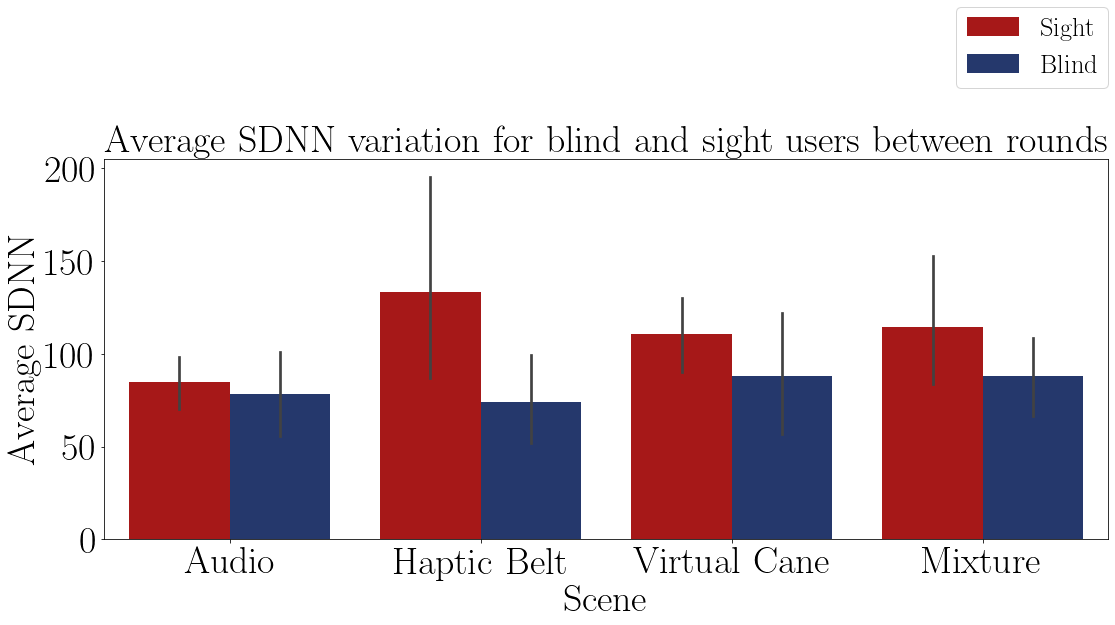
\includegraphics[width = 0.8\linewidth]{Resultados/ECG/Figuras/pdf/barplot_ecg_sdnn_4_scene.pdf}
%    \caption{Barplot of the average SDNN of both participants on each method.}
%    \label{fig:barplot_ecg_sdnn_4_scene}
%\end{figure}

No clear pattern is evident from this figure. For some methods, the return round resulted in a decrease in the SDNN, while for others, it increased. 

Figures \ref{fig:boxplot_ecg_sdnn_4_scene} and \ref{fig:boxplot_ecg_sdnn_4_rounds} shows the boxplots for both groups. Both pictures show that the SDNN of the sighted users was higher than that of the blind users, indicating that sighted users had a lower mental workload than the blind users.

\begin{figure}[!htb]
    \centering
    \begin{minipage}{0.45\textwidth}
        \centering
        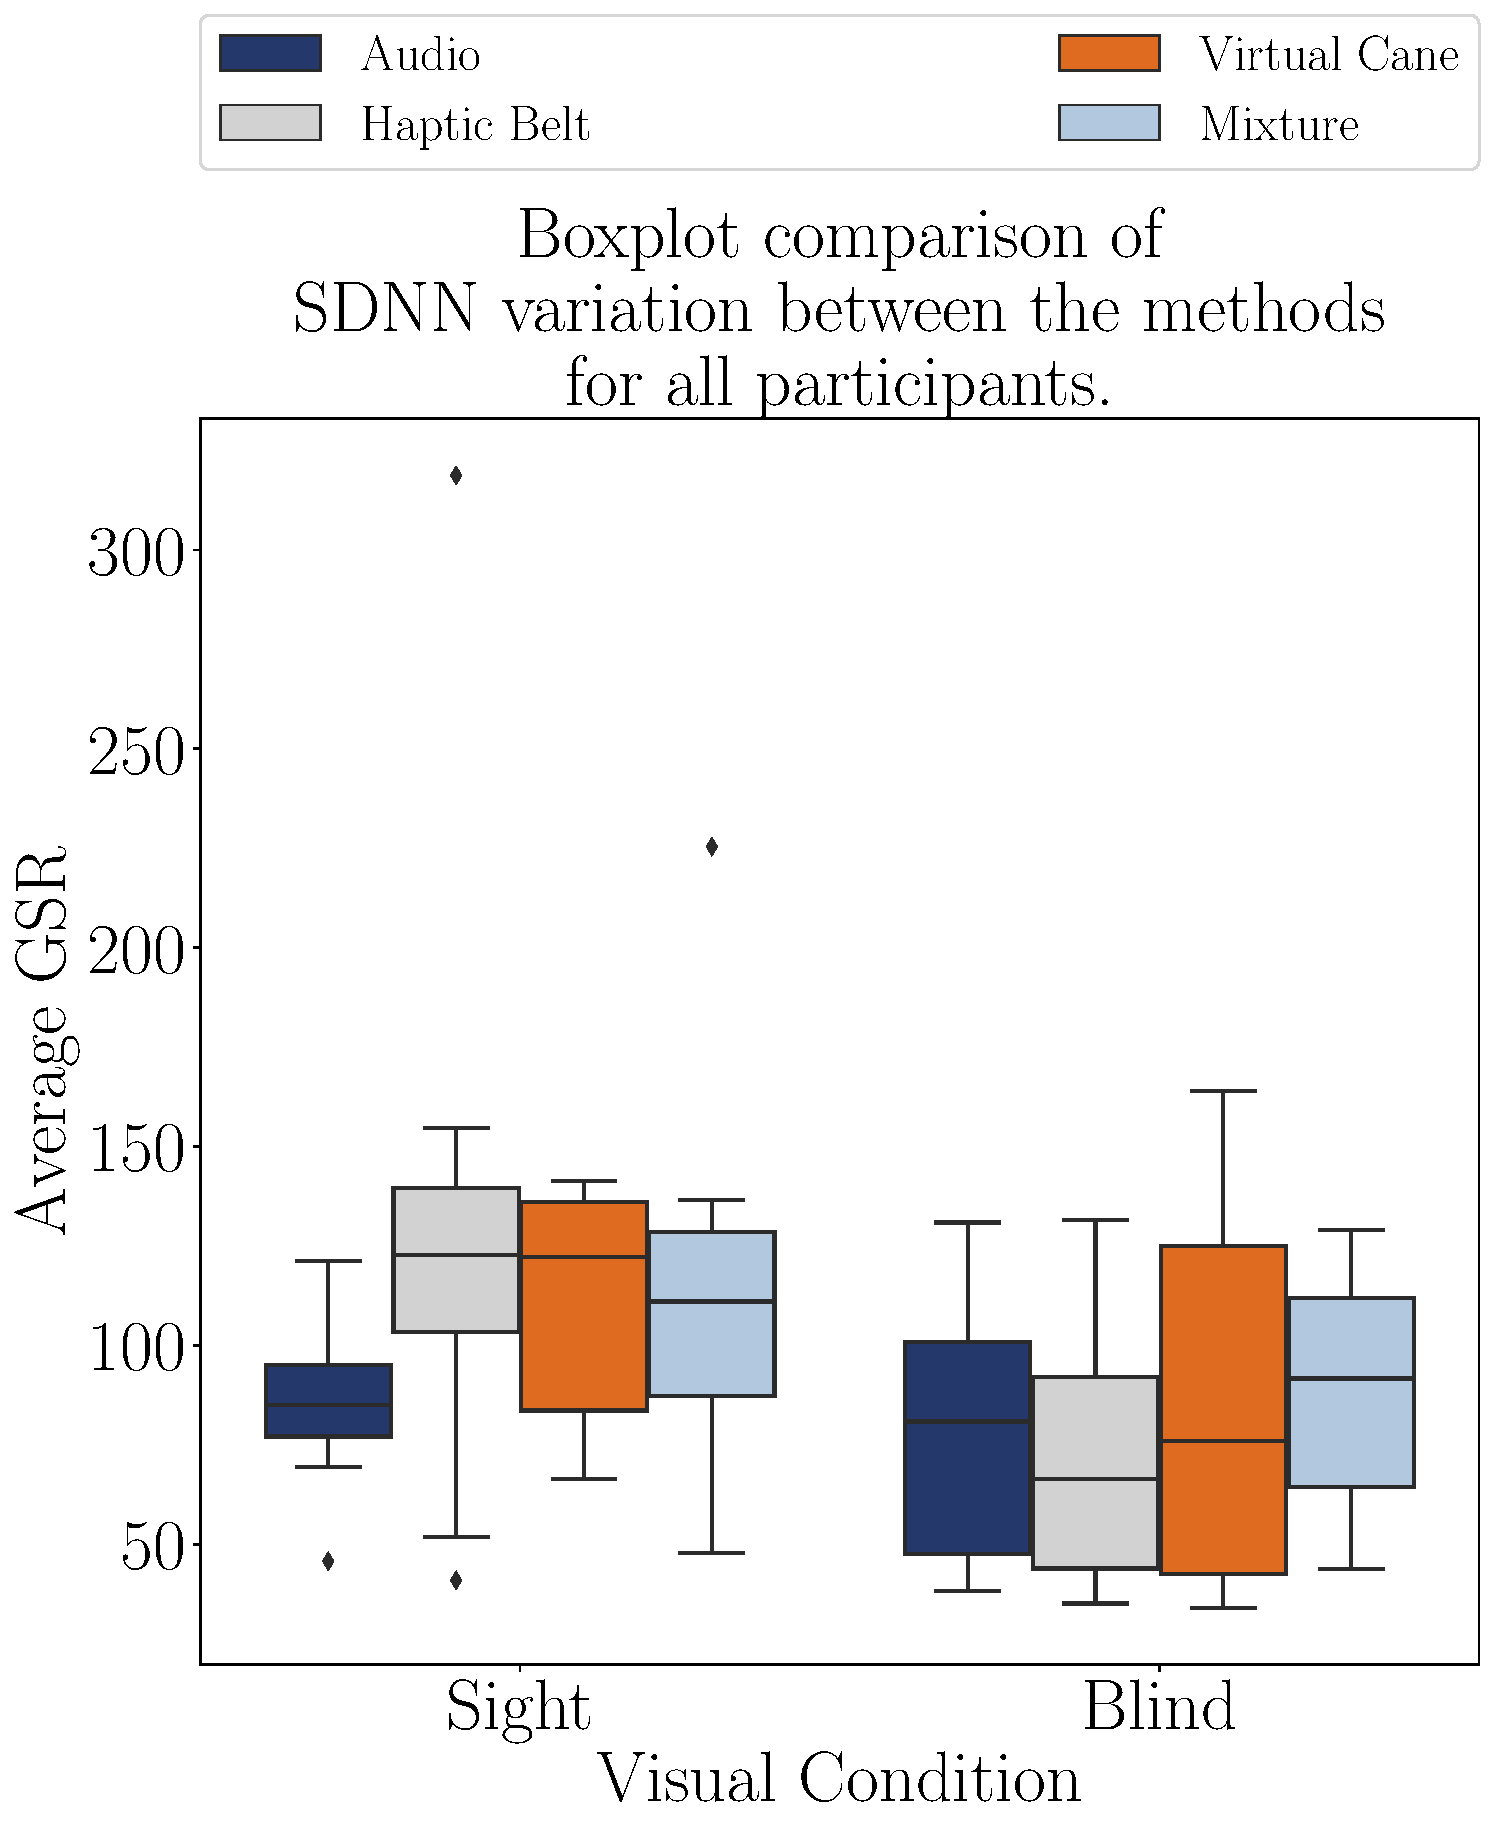
\includegraphics[width = \textwidth]{Resultados/ECG/Figuras/pdf/boxplot_ecg_sdnn_4_scene.pdf}
        \caption{Boxplot of the average SDNN of the participants grouped by the methods.}
        \label{fig:boxplot_ecg_sdnn_4_scene}
    \end{minipage}
    \begin{minipage}{0.075\textwidth}
        \hfill
    \end{minipage}
    \begin{minipage}{0.45\textwidth}
        \centering
        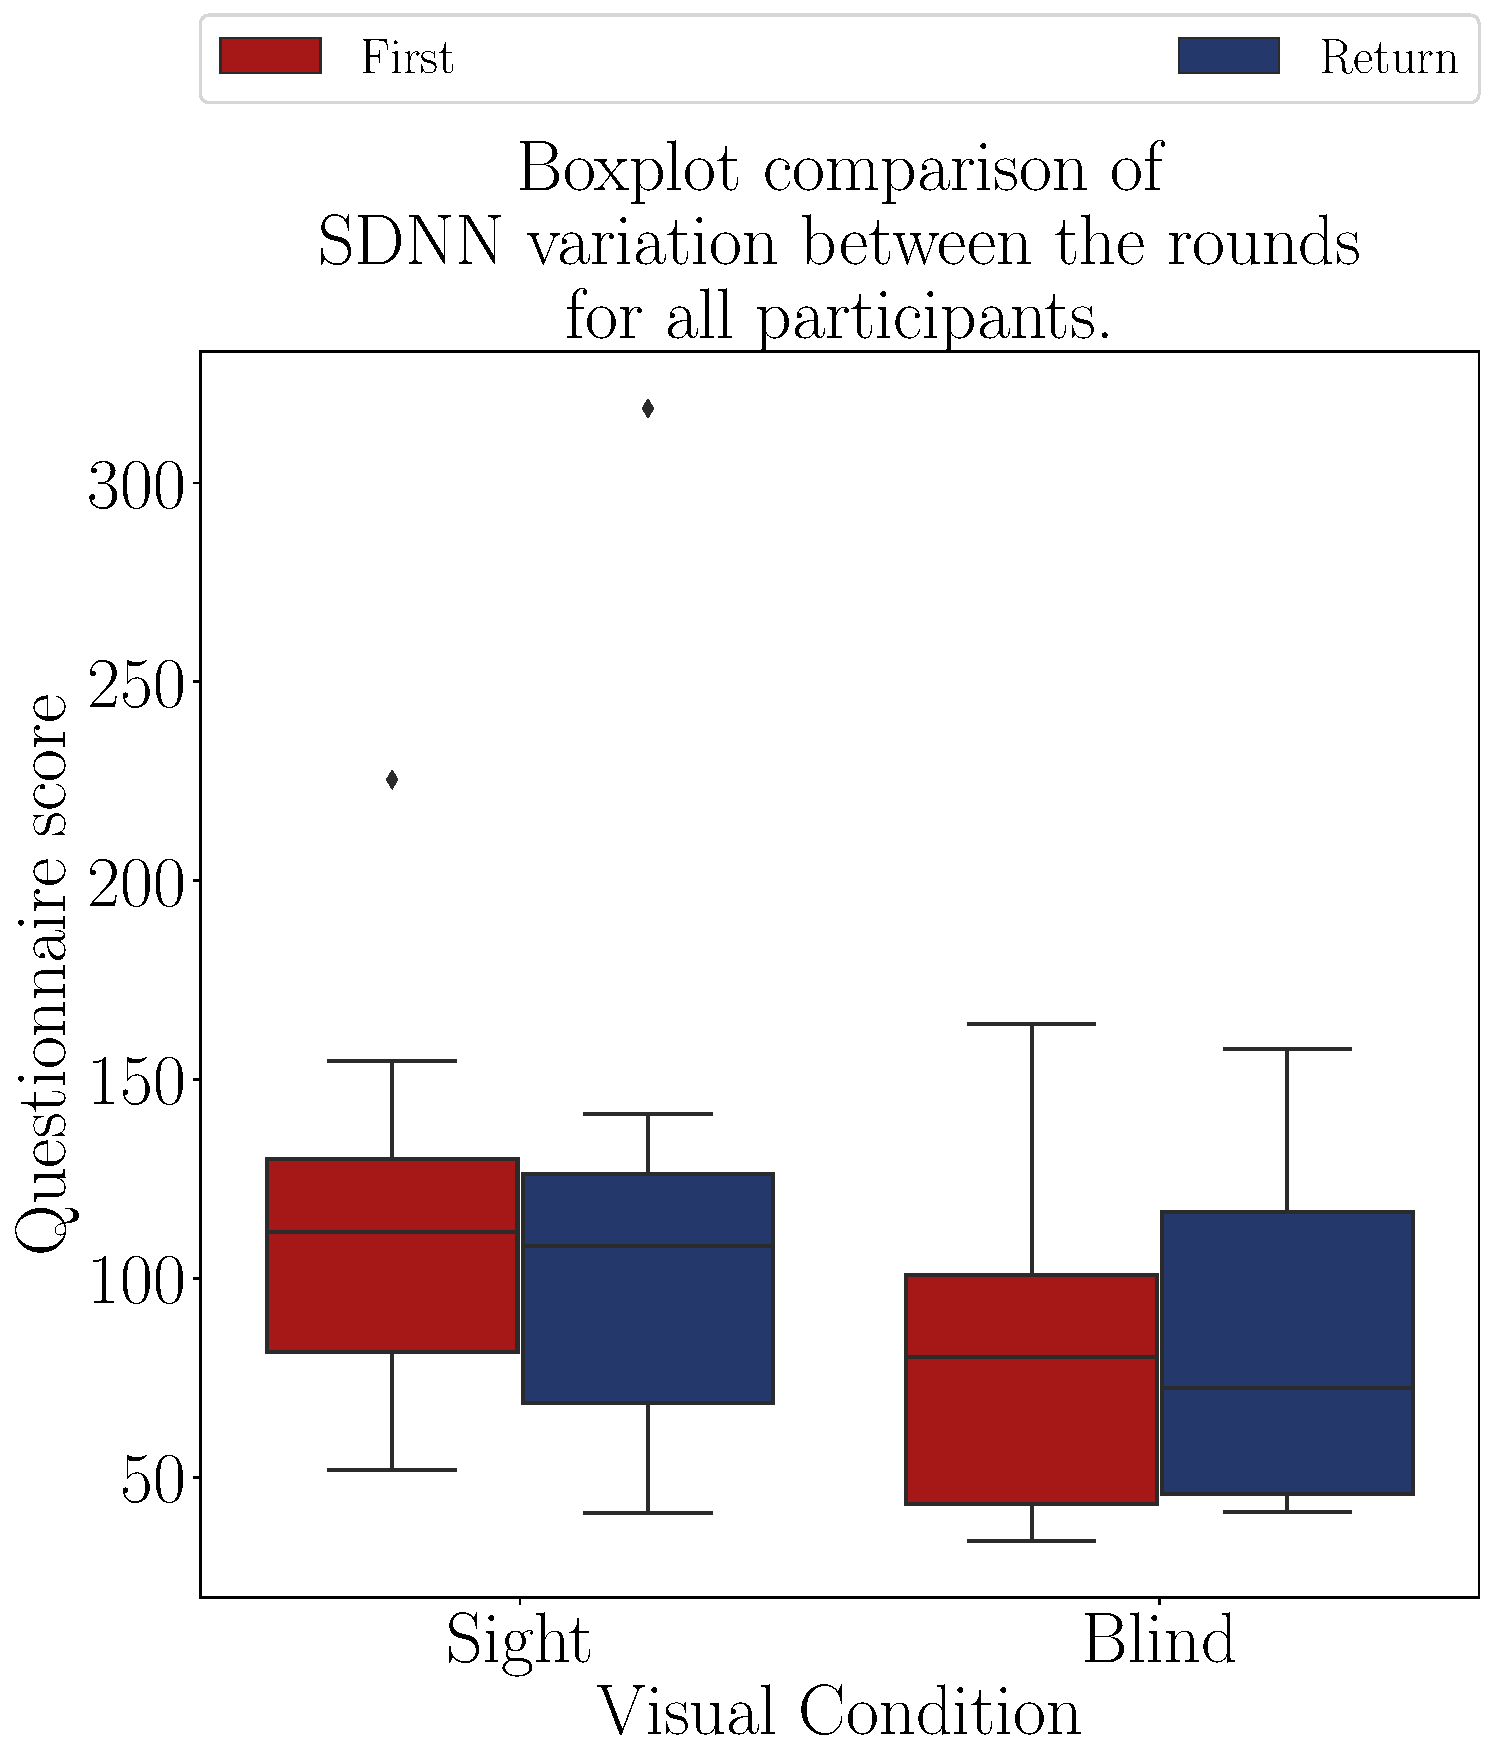
\includegraphics[width = \textwidth]{Resultados/ECG/Figuras/pdf/boxplot_ecg_sdnn_4_rounds.pdf}
        \caption{Boxplot of the average SDNN of the participants grouped by the rounds.}
        \label{fig:boxplot_ecg_sdnn_4_rounds}
    \end{minipage}
\end{figure}
 
%The Table \ref{tab:sdnn_average_group_noBase} shows the average heartbeat variance of both samples and is possible to notice how the average score by the sight users was higher in every method, reinforcing the Figures \ref{fig:barplot_ecg_sdnn_4_scene} to \ref{fig:boxplot_ecg_sdnn_4_rounds} conclusions.
%
%
\begin{table}[!htb]
\centering
\caption{ECG Average SDNN average in relation to the baseline grouped by participant and visual Condition.}
\label{tab:sdnn_average_group_noBase}
\begin{tabular}{lllrrrr}
\toprule
{} &  Audio & Haptic Belt & Virtual Cane & Mixture \\
Visual Condition &        &             &              &         \\
\midrule
Blind            &  78.46 &       74.03 &        88.32 &   88.13 \\
Sight            &  84.92 &      133.33 &       110.53 &  114.33 \\
\bottomrule
\end{tabular}
\end{table}



Figures \ref{fig:qqplot_sdnn_two_way_sight} and \ref{fig:residplot_sdnn_two_way_sight} bring the QQ Plot and residual distribution. Figure \ref{fig:qqplot_sdnn_two_way_sight} hints that the data from sighted users contain two outliers. Table \ref{tab:blocanova_sdnn_two_way_blind_sight} shows the ANOVA test p-values. For both groups, none of the factors have a significant influence on the SDNN value.

\begin{table}[!htb]
    \caption{Anova p-value for the average SDNN on each method.'}
    \label{tab:blocanova_sdnn_two_way_blind_sight}
\begin{minipage}{0.45\textwidth}
    \subcaption{Blind participants}
    \input{Resultados/ECG/Tabelas/blocanova_sdnn_two_way_blindsemBegin.tex}
\end{minipage}
\begin{minipage}{0.45\textwidth}
    \subcaption{Sight participants}
    \input{Resultados/ECG/Tabelas/blocanova_sdnn_two_way_sightsemBegin.tex}
\end{minipage}
\end{table}

\begin{figure}[!htb]
    \centering
    %\vspace{-15.0cm}
    \begin{minipage}{0.45\textwidth}
        \centering
        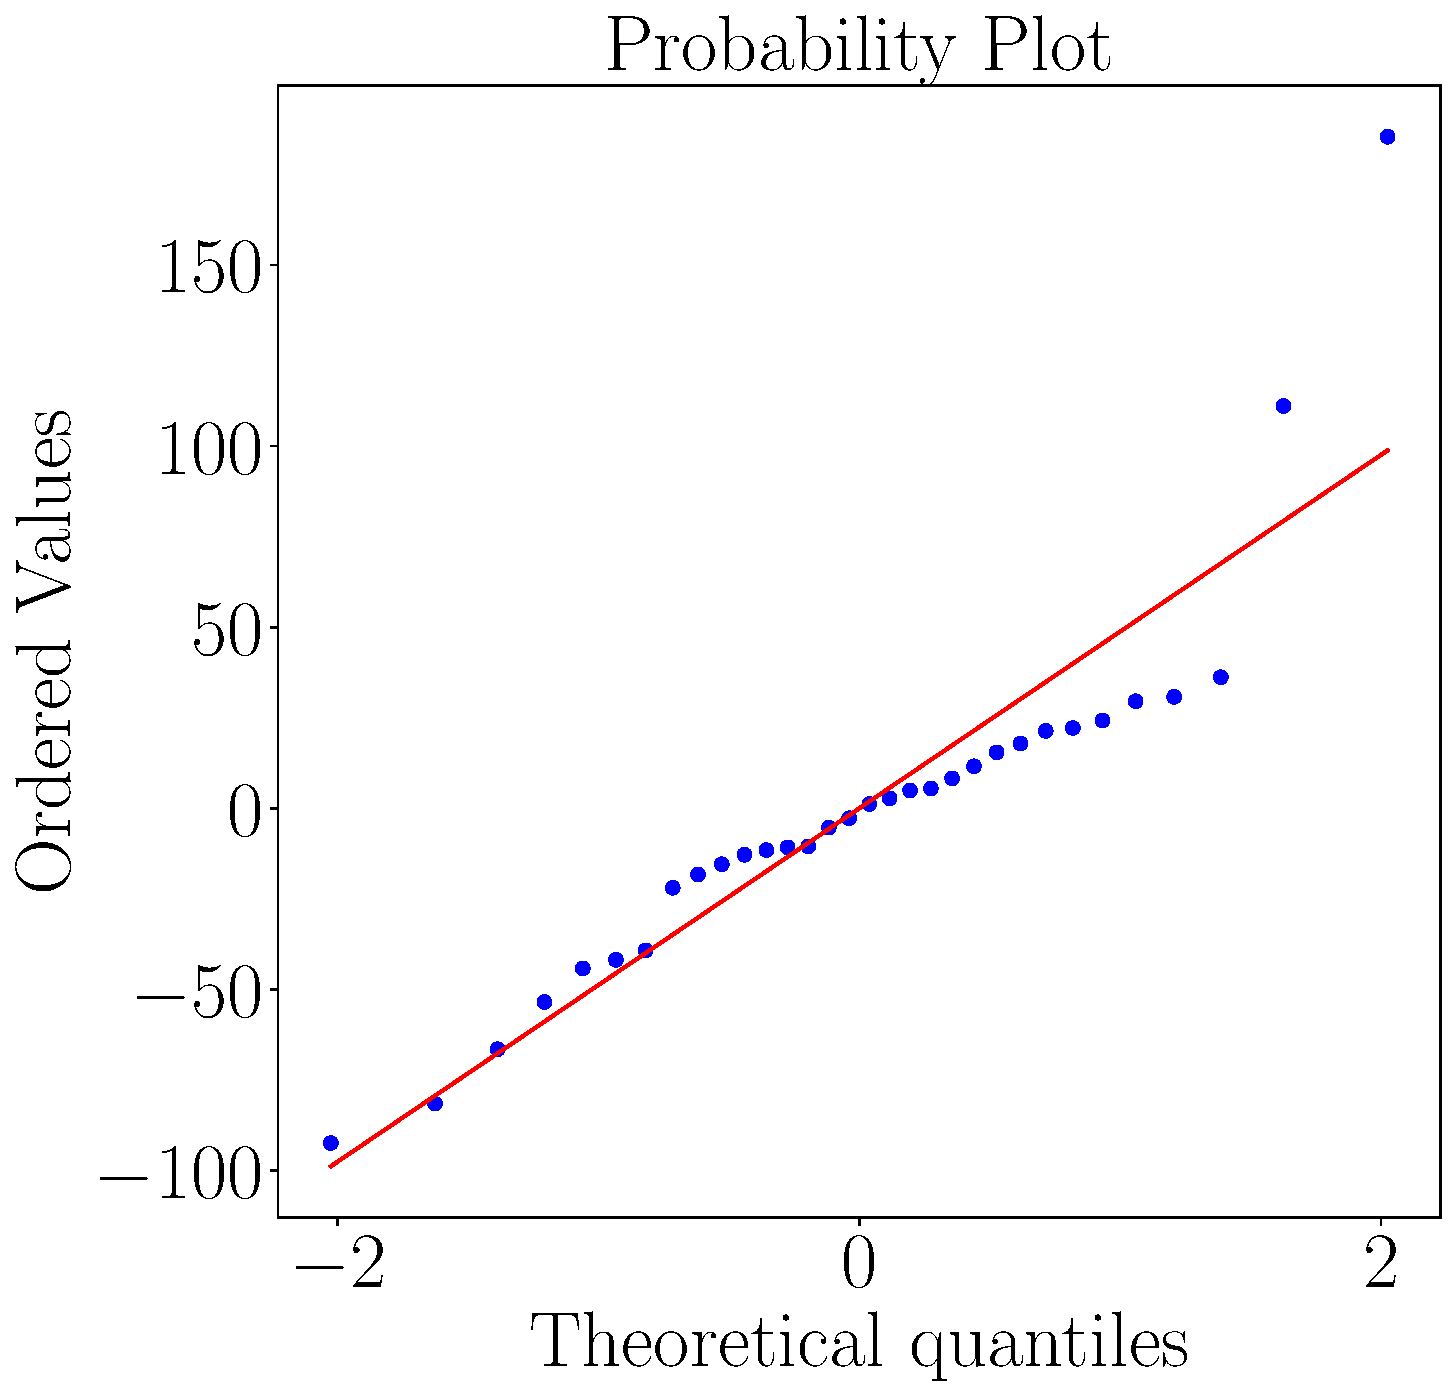
\includegraphics[width = \textwidth]{Resultados/ECG/Figuras/pdf/qqplot_sdnn_two_way_sight.pdf}
        \caption{QQ plot of the average SDNN of the sight participants on each method.}
        \label{fig:qqplot_sdnn_two_way_sight}
    \end{minipage}
    \begin{minipage}{0.075\textwidth}
        \hfill
    \end{minipage}
    \begin{minipage}{0.45\textwidth}
        \centering
        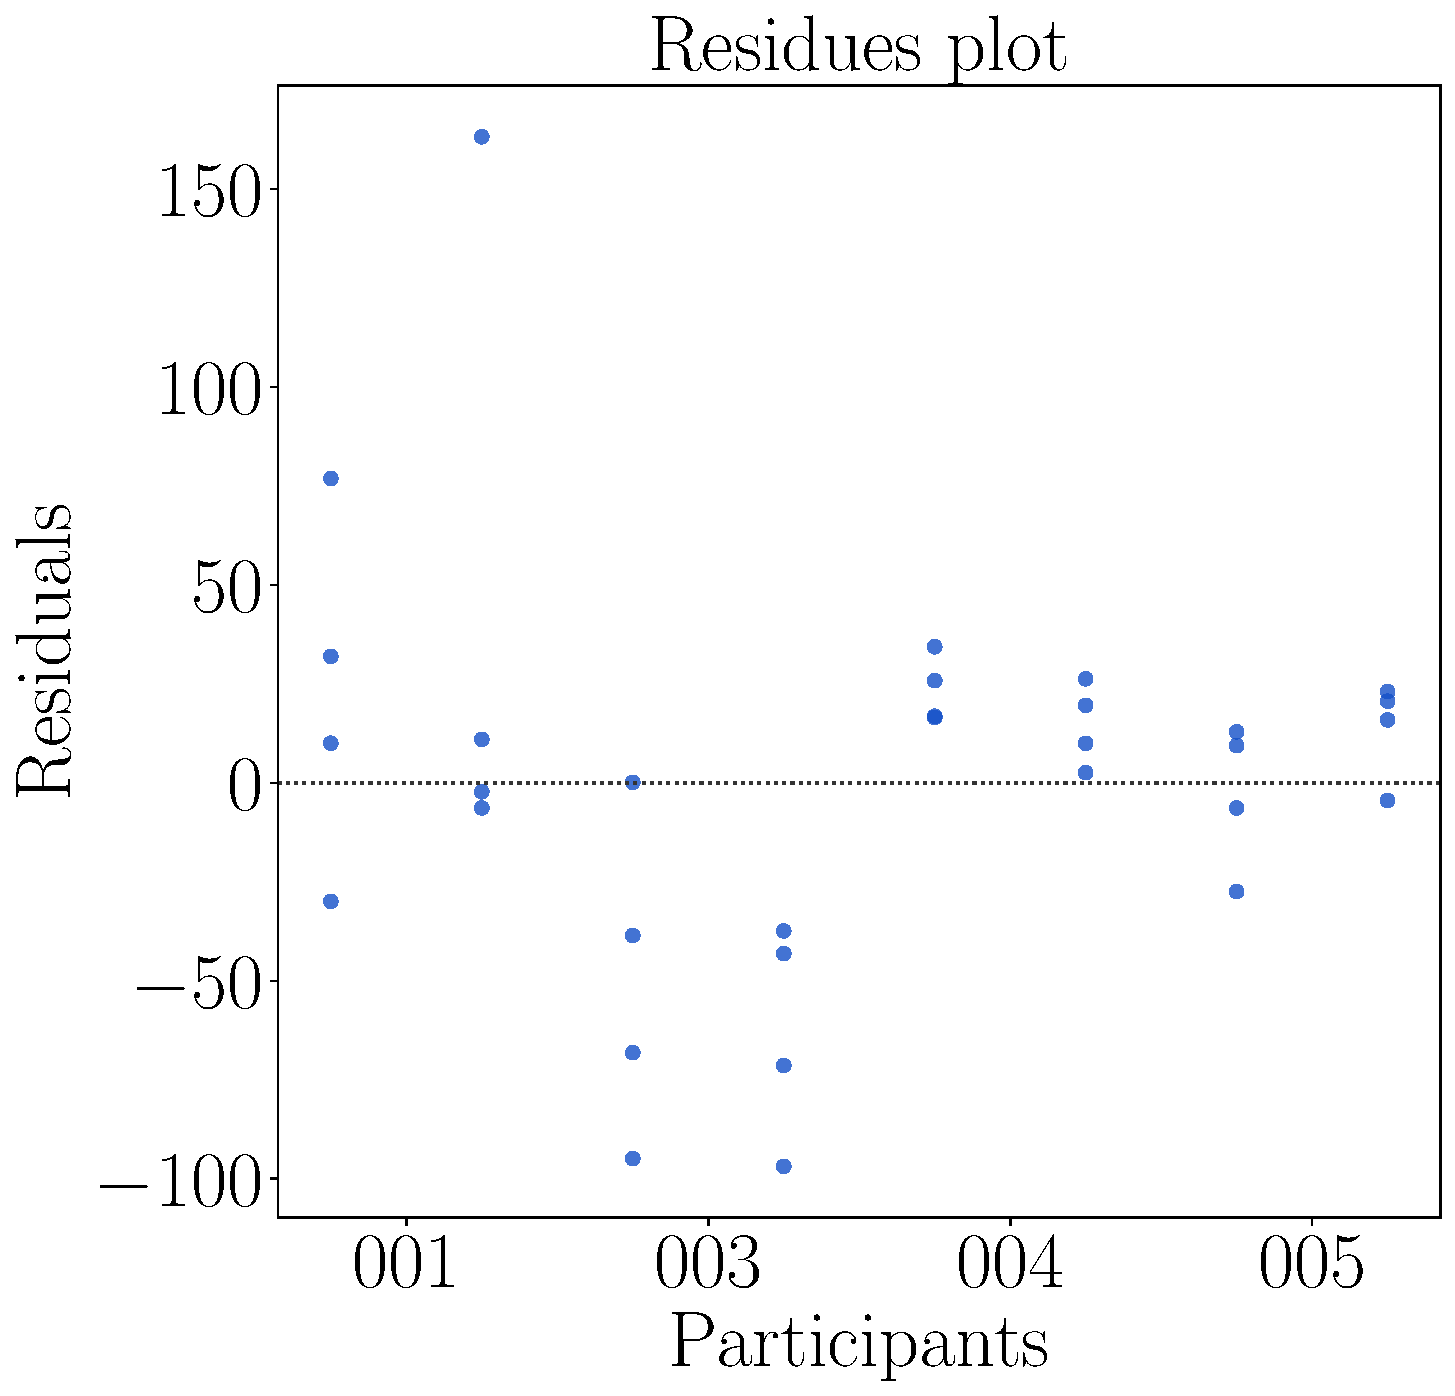
\includegraphics[width = \textwidth]{Resultados/ECG/Figuras/pdf/residplot_sdnn_two_way_sight.pdf}
        \caption{Residual plot of the average SDNN score the sight participants on each method.}
        \label{fig:residplot_sdnn_two_way_sight}
    \end{minipage}
\end{figure}


%
\begin{table}[!htb]
\centering
\caption{Cross validation p-value for the average SDNN on each method for blinded users.}
\label{tab:lsd_sdnn_two_way_sight}
\begin{tabular}{rclr}
\toprule
      \multicolumn{3}{c}{Method} &                          \multicolumn{2}{c}{Analysis} \\
\midrule
       Audio & $X$ & Haptic Belt &        $H_1 : \mu_{Audio} \ne \mu_{Haptic Belt}$ & ** \\
      Audio & $X$ & Virtual Cane &       $H_1 : \mu_{Audio} \ne \mu_{Virtual Cane}$ & ** \\
           Audio & $X$ & Mixture &            $H_1 : \mu_{Audio} \ne \mu_{Mixture}$ & ** \\
Haptic Belt & $X$ & Virtual Cane & $H_1 : \mu_{Haptic Belt} \ne \mu_{Virtual Cane}$ & ** \\
     Haptic Belt & $X$ & Mixture &      $H_1 : \mu_{Haptic Belt} \ne \mu_{Mixture}$ & ** \\
    Virtual Cane & $X$ & Mixture &         $H_0 : \mu_{Virtual Cane} = \mu_{Mixture}$ &  \\
\bottomrule
\end{tabular}
\end{table}


%
%The Table \ref{tab:lsd_sdnn_two_way_sight} presents the conclusion of a pairwise Fisher LSD test of the blind heart rate frequency variation between all the guidance methods and it shows that all methods had different effect on the heartrate, appart of the "Virtual Cane" and "Mixture", which presented similar SDNN.

%According to the ANOVA test at Table \ref{tab:blocanova_sdnn_two_way_sight} there was no effect on the interbeat variance. So the methods did not influence the sighted user mental workload. The same conclusion was driven in the section \ref{subsubsec:results_ecg_1} in the SDNN part.
%
%Also, the sight user had a higher SDNN, which means lower Mental Workload, a unexpected result based on the expectation and on the previous notes. 

\FloatBarrier